% \section{Introduction}
% Todo: Introduction structure
% 0) we introduce & define the problem 1) we survey which techniques
% exist 2) we implement (for a lack of readily available implementations)
% and compare the most promising ones 3) we draw conclusions for when to
% use which technique


% TODO: Include term predictive CI, link to FB paper and
%https://www-sciencedirect-com.tudelft.idm.oclc.org/science/article/pii/S0164121218301730

% TODO: What about the alternate solution, installing plugins to report
% precise data? Ie., maven plugins
% - Lots of effort
% - not a generic solution
% - how to analyze history where such plugins were not installed
% - unclear which information you want

% TODO It would be futile to compare our techniques with one of the
% existing manual regex parsers, as (a) as our literature survey showed,
% their scope is mainly limited to the Java ecosystem and (b) whether
% they would work or not would be randomly based on whether the project
% we select exhibits features their regular expressions were trained for.
% Finally, they are not really automatic

\lstset{
  morekeywords={},
	basicstyle=\ttfamily\scriptsize,
  postbreak=\mbox{\textcolor{blue}{$\hookrightarrow$}\space},
  showspaces=false,
  showstringspaces=false,
  stringstyle=\color{Plum},
	frame=single,
  extendedchars=false,
  texcl=false,
  aboveskip=\baselineskip,
  belowskip=0pt
}

Continuous Integration (CI) has become a common practice in software
engineering~\cite{hilton2016usage}.
Many software projects use
CI~\cite{hilton2016usage,staahl2014modeling,beller2017oops} to detect
bugs early~\cite{vasilescu2015quality,duvall2007continuous}, improve
developer productivity~\cite{miller2008hundred,hilton2016usage} and
communication~\cite{downs2012ambient}.
CI builds produce logs which
report results of various sub-steps within the build.
These build logs
contain a lot of valuable information for developers and researchers---for
example, descriptions of compile errors, linter warnings or failed
tests~\cite{beller2017oops,seo2014programmers,vassallo2017a-tale}.

CI builds produce logs which report the results of the steps within
the build.
The information stored in build logs can and has
already been used for a variety of applications.
One prominent dataset
in the space, TravisTorrent, was featured as the MSR Data Challenge
2017~\cite{msr17challenge}.
To date, scientist and practitioners alike
have used it and other, proprietary datasets to understand and
cateogrize Continuous Integration build
failures~\cite{islam2017insights}, to do research on testing
practices~\cite{orellana2017differences}, to train classifiers to
predict the build outcome and
duration~\cite{ni2017cost,bisong2017built,machalica2019predictive},
and to investigate static analysis tools in CI
builds~\cite{zampetti2017open}.
Therefore, being able to efficiently
and correctly extract information from build logs is paramount to the
future of a variety of fields depending on it.

However, build logs can be verbose and large---sometimes in excess of
50 MB of ASCII text~\cite{beller2017oops}---making them inadequate
for direct human consumption.
Therefore, to support developers and
researchers in efficiently making use of the information within build
logs, we must at least semi-automatically retrieve the chunks of the
log that describe the targeted information.

There are different techniques to retrieve information chunks from CI
build logs.
Beller et al.\ use a rule-based system of regular
expressions to analyze logs from Travis CI~\cite{beller2017oops}.
Such regular expressions are developed by looking at exemplary build
logs.
Vassallo et al.\ wrote a custom parser to gather information
for build repair hints~\cite{vassallo2018un-break}.
Recently, Amar et
al.\ reduced the number of lines for a developer to inspect by
creating a diff between logs from failed and successful
builds~\cite{amar2019mining}.

These approaches have various strengths and weaknesses: Regular
expressions are exact, but tedious and error-prone to
maintain~\cite{michael2019regexes}.
Custom parsers are powerful
though fragile in light of changes in the log structure.
Diffing
between failed and successful logs can reduce the information to be
processed, but is at best semi-automatic~\cite{amar2019mining}.

% TODO: 4 sentence description of the steps in graphic?
\Cref{fig:overview} gives an overview of our research steps.
We conducted a systematic mapping study,
to gain an impression on how researchers are using information from
build logs within their research or to support
developers.
% We implemented three promising techniques that retrieve
% chunks of text from build logs and can be adapted to
% a specific project and use case by giving examples of build logs and
% correpsonding chunks.
% We evaluated the
Our goal was to clarify the state-of-research on build log
analysis (\textbf{RQ1}).

The outcomes of our study shows that there are various attempts to
retrieve specific information from buildlogs.
The resulting implementations are rarely available and therefore rarely
reused.
Because of the high development overhead
of the custom parsers, many implementations are limited to small number
of supported build tools.

\begin{figure*}[htb]
	\centering
	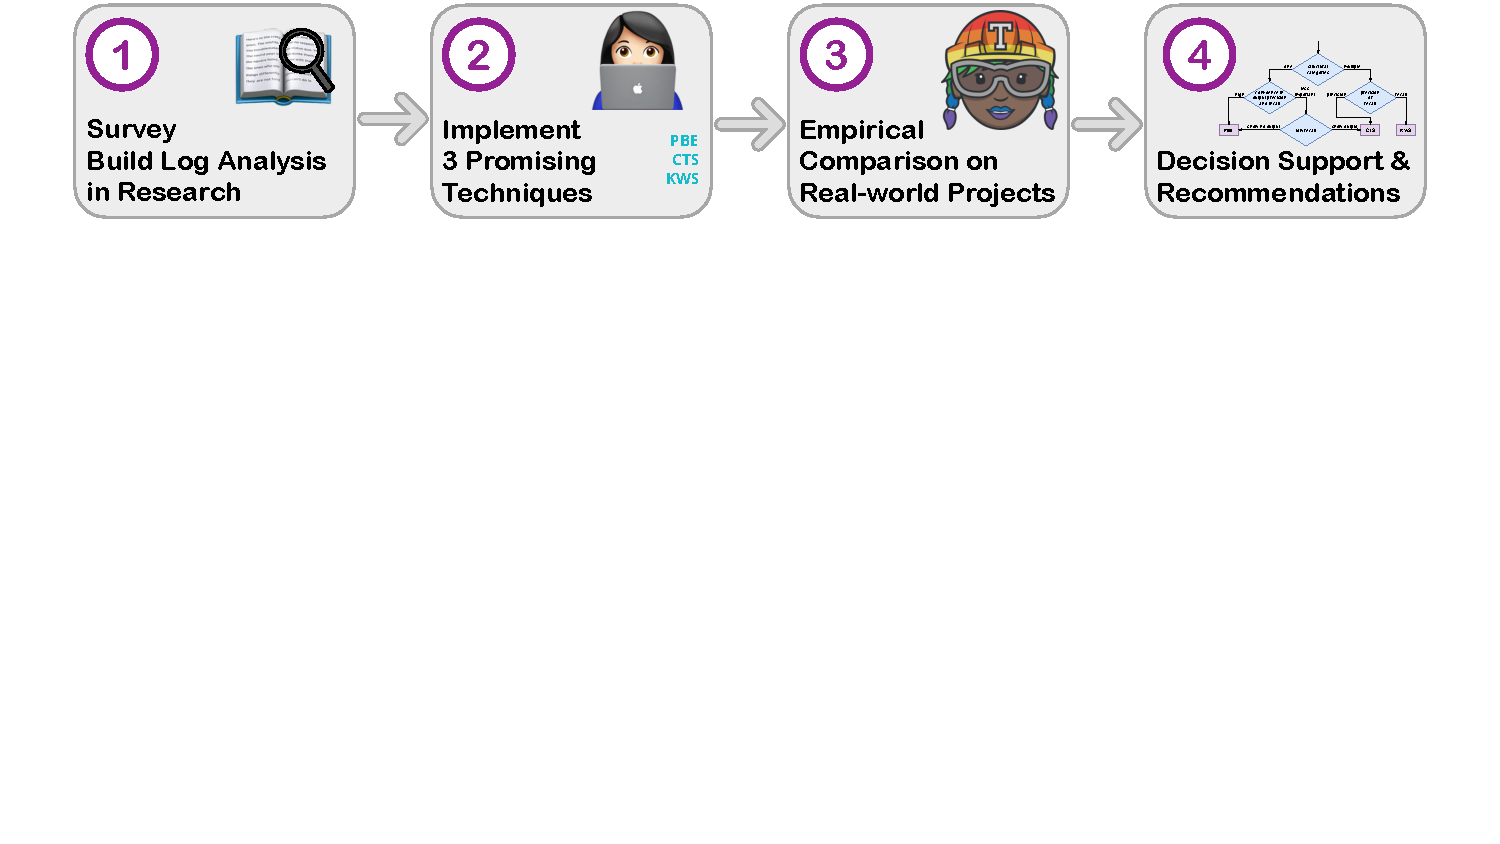
\includegraphics[width=\textwidth, trim={1.2cm 10.5cm 1.2cm 0cm},
	clip]{img/overview.pdf}
	\caption{Our Research Workflow.}
	\label{fig:overview}
\end{figure*}

To address this, we implement three promising techniques for build
log analysis.
They retrieve specific chunks of targeted information and are trained
with examples provided by the user.
We conduct an empirical study on the \emph{LogChunks} data
set~\cite{brandt2020logchunks} to
gauge the performance of these chunk retrieval techniques and characterize
when one of the techniques should be preferred over other alternatives
(\textbf{RQ2}).

\begin{simplebox}[minipage boxed title*=-5cm]{Research Questions}
\begin{itemize}
  \item[\textbf{RQ1:}] What is the state-of-research on build
  log analysis?
  \item[\textbf{RQ2:}] When are PBE, CTS or KWS suited to
  retrieve chunks from build logs?
\end{itemize}
\end{simplebox}

% also moved down to where mentioned in detail
% left copy here for convenience

% \begin{simplebox}[attach boxed title to top center={yshift=-6mm}]
% {\textbf{RQ1:} What is the state-of-research on build
% log analysis?}
% \begin{itemize}
%   \item[\textbf{RQ1.1:}] Which information is targeted?
%   \item[\textbf{RQ1.2:}] Which techniques are used?
%   \item[\textbf{RQ1.3:}] Which build logs are analyzed?
% \end{itemize}
% \end{simplebox}

% \begin{simplebox}[minipage boxed title*=-2.5cm,
% attach boxed title to top center={yshift=-6mm}]
% {\textbf{RQ2:} When are PBE{,} CTS or KWS suited to
% retrieve chunks from build logs?}
% \begin{itemize}
%   \item[\textbf{RQ2.1:}] How many examples does a technique need to
%   perform best?
%   \item[\textbf{RQ2.2:}] How structurally similar do the examples
%   need for a technique to be applicable?
%   \item[\textbf{RQ2.3:}] How accurate are the retrievals of a technique?
% \end{itemize}
% \end{simplebox}


% % At the moment there is only anecdotal evidence on the performance
% of these
% % techniques and on when a technique should be preferred over other
% alternatives.
% % Developers and researches currently have little support when choosing
% which
% % technique to use for a task.

% % The goal of this article is to investigate different chunk retrieval
% techniques
% % for build logs and describe under which circumstances certain
% techniques
% can be
% % recommended over others.
% % We aim to characterize different chunk retrieval techniques.
% % For \textbf{Research Question 1} (\textbf{RQ1}), we analyze which
% criteria
% % influence the suitability of a chunk retrieval technique for CI
% build logs.

We implement and evaluate three chunk retrieval techniques:
\begin{itemize}
  \item \textbf{Program Synthesis by Example (referred to as PBE)}
  Based on user examples of build logs and chunks, PBE
  synthesizes
  a regular expression matching the given chunks within the build logs.
  \item \textbf{Common Text Similarity (CTS)}
  Using the Vector Space Model, CTS selects those lines of a log which are
  most similar to the lines present in example chunks provided by
  the user.
  \item \textbf{Keyword Search (KWS)}
  Ad-hoc method for finding fitting passages by searching the whole
  text for
  the occurrence of specific trigger words.
\end{itemize}

Following the results from our comparison study,
recommend PBE for use cases where the desired information is always
represented in the same structural way and high confidence in precision
and recall of the chunk retrieval is required.
Results produced by PBE are suited for automatic on-ward processing.
CTS is well suited when the representation of the desired information
varies
slightly and the output of the chunk retrieval is further processed by
a human.
In cases where the textual representation of the desired information in
the log
is unpredictable or varies greatly, KWS seems to be the best choice.
However,
its low precision---it extracts a context of multiple lines around a
finding---makes it generally unsuited for automatic on-ward processing and
instead requires a human to further inspect and interpret the output
chunk.

\begin{figure*}[!t]
  \centering
\begin{subfigure}[t]{\columnwidth}
  \begin{lstlisting}[breaklines=true,frame=tlr]
FAILURE: Build failed with an exception.

* What went wrong:
  \end{lstlisting}
  \vspace{-\baselineskip}
  \begin{lstlisting}[backgroundcolor=\color{Cerulean!60},breaklines=true,frame=rl]
Could not determine the dependencies of task ':app:jacocoTestDebugReport'.
> Task with path 'testDebug' not found in project ':app'.
  \end{lstlisting}
  \vspace{-\baselineskip}
  \begin{lstlisting}[breaklines=true,frame=blr]

* Try:
  \end{lstlisting}
\end{subfigure}\hspace{\fill}
\begin{subfigure}[t]{\columnwidth}
  \centering
  \begin{lstlisting}[breaklines=true,frame=tlr]
FAILURE: Build failed with an exception.

* What went wrong:
  \end{lstlisting}
  \vspace{-\baselineskip}
  \lstinputlisting[backgroundcolor=\color{Cerulean!60},breaklines=true,frame=rl]{listings/chunk1.txt}
  \vspace{-\baselineskip}
  \begin{lstlisting}[breaklines=true,frame=blr]

* Try:
  \end{lstlisting}
\end{subfigure}
  \caption{Two examples of log chunks explaining why an Android
  build failed.}
  % TODO Moritz: we can relate this to travistorrent maybe, you told me
  % long ago that this was something your analyzer cannot extract
  \label{lst:chunk-example}
\end{figure*}

\lstset{language=caml, morekeywords={StartExtraction, RegexPosition,
RegexPair,
  EndExtraction}, keywordstyle=\bfseries\color{black}, escapeinside=//}
\begin{figure}[!t]
  \centering
  \lstinputlisting[breaklines=true]{listings/prose.txt}
  \caption{Simiplified regular expression produced by PBE when trained
  with examples from \Cref{lst:chunk-example}}
  \label{lst:prose-program-simplified}
\end{figure}

\lstset{
  language=,
  morekeywords={},
  texcl=false
}
\begin{figure}[!t]
  \centering
  \begin{lstlisting}[breaklines=true,frame=tlr]
=== RUN   TestSeparator
  \end{lstlisting}
  \vspace{-\baselineskip}
  \lstinputlisting[backgroundcolor=\color{Cerulean!60},breaklines=true,frame=rl]{listings/chunk2.txt}
  \vspace{-\baselineskip}
  \begin{lstlisting}[breaklines=true,frame=blr]
=== RUN   TestGenerateHTML
  \end{lstlisting}
  \caption{Example of a log chunk showing a linter error}
  \label{lst:chunk-example-3}
\end{figure}

% TODO: this could move to the chunk retrieval techniques section
The results of our empirical comparison study on the chunk retrieval
techniques
show that the structural representation of the targeted chunk greatly
influences
the performance of the chunk retrieval techinques.
\Cref{lst:chunk-example} shows two exemplary
log chunks from Android build logs marked in blue.
Both chunks contain the information on why the
corresponding build failed.
When PBE is trained with these two examples it produces
a regular expression program similar to the one presented in
\Cref{lst:prose-program-simplified}.
The retrieval
starts after a colon and a line separator and before a capital
letter.
It ends before two line separators, consistent with the two example
chunks from \Cref{lst:chunk-example}.
This shows, that the characters structuring the text around the chunk are
cruicial for regular expressions to identify a log chunk.
In fact, if the third example from \Cref{lst:chunk-example-3} with a
different structural representation is added to the training set,
PBE is not able to syntesize a program and returns
``\texttt{no program found}''.
We express this difference in structural representation through
dividing log chunks into structural categories.
The chunks from \Cref{lst:chunk-example}
are in the \emph{same structural category}, while the chunk from
\Cref{lst:chunk-example-3} is in a \emph{different structural category}.


% % \textbf{RQ2} asks under which conditions PBE, CTS and KWS are suited
% to retrieve information from continuous integration build logs.
% % \textbf{RQ2} is refined into sub-questions along with the criteria
% resulting from \textbf{RQ1} and compares their instantiations for the
% three techniques:
% % how many training examples a technique needs to perform best
% (\textbf{RQ2.1}), how structurally diverse the examples can
% be (\textbf{RQ2.2}) and how accurate the retrieved output is
% (\textbf{RQ2.3}).
% % To evaluate PBE, CTS and KWS we use the \emph{LogChunks} data set,
% which encompasses about 800 log files from 80 repositories.
% % Each log is labeled with the log part describing the reason a build
% failed, keywords to search for this log part and a categorization of
% the labeled log part according to its structural representation within
% the log.

% Our study of the three techniques on \emph{LogChunks} shows that
% \begin{itemize}
%   \item PBE yields very accurate results when trained with two examples
%   from a
%   single structural category.
%   \item CTS shows the best average precision, though precision and
% recall
%   of a
%   retrieval is hard to determine from the given result.
%   A small increase in the number of training examples has no noticeable
%   influence.

%   Fewer structural categories improve precision and recall of the
%   retrieval.
%   \item KWS has the highest recall of all techniques, however much
%   lower precision.
%   It is the technique with the best recall when multiple structural
%   categories
%   are present in the training examples.
% \end{itemize}

% % \noindent
% % \textbf{Our work contributes:}
% % \begin{itemize}
% %   \item A tool with three prototypical implementations of chunk
% retrieval techniques:
% %	  \begin{itemize}
% %	    \item program synthesis from examples using the Microsoft
% PROSE library (PBE),
% %	    \item a common information retrieval approach using text
% similarity (CTS), and
% %	    \item a keyword search approach (KWS).
% %	  \end{itemize}
% %   \item Recommendations for the configuration of each of the
% investigated chunk retrieval techniques.
% %   \item Guidelines on choosing a suitable chunk retrieval technique.
% % \end{itemize}


\section{Systematic Literature Mapping Survey}
\label{sec:survey}

\begin{figure}[hb]
	\centering
	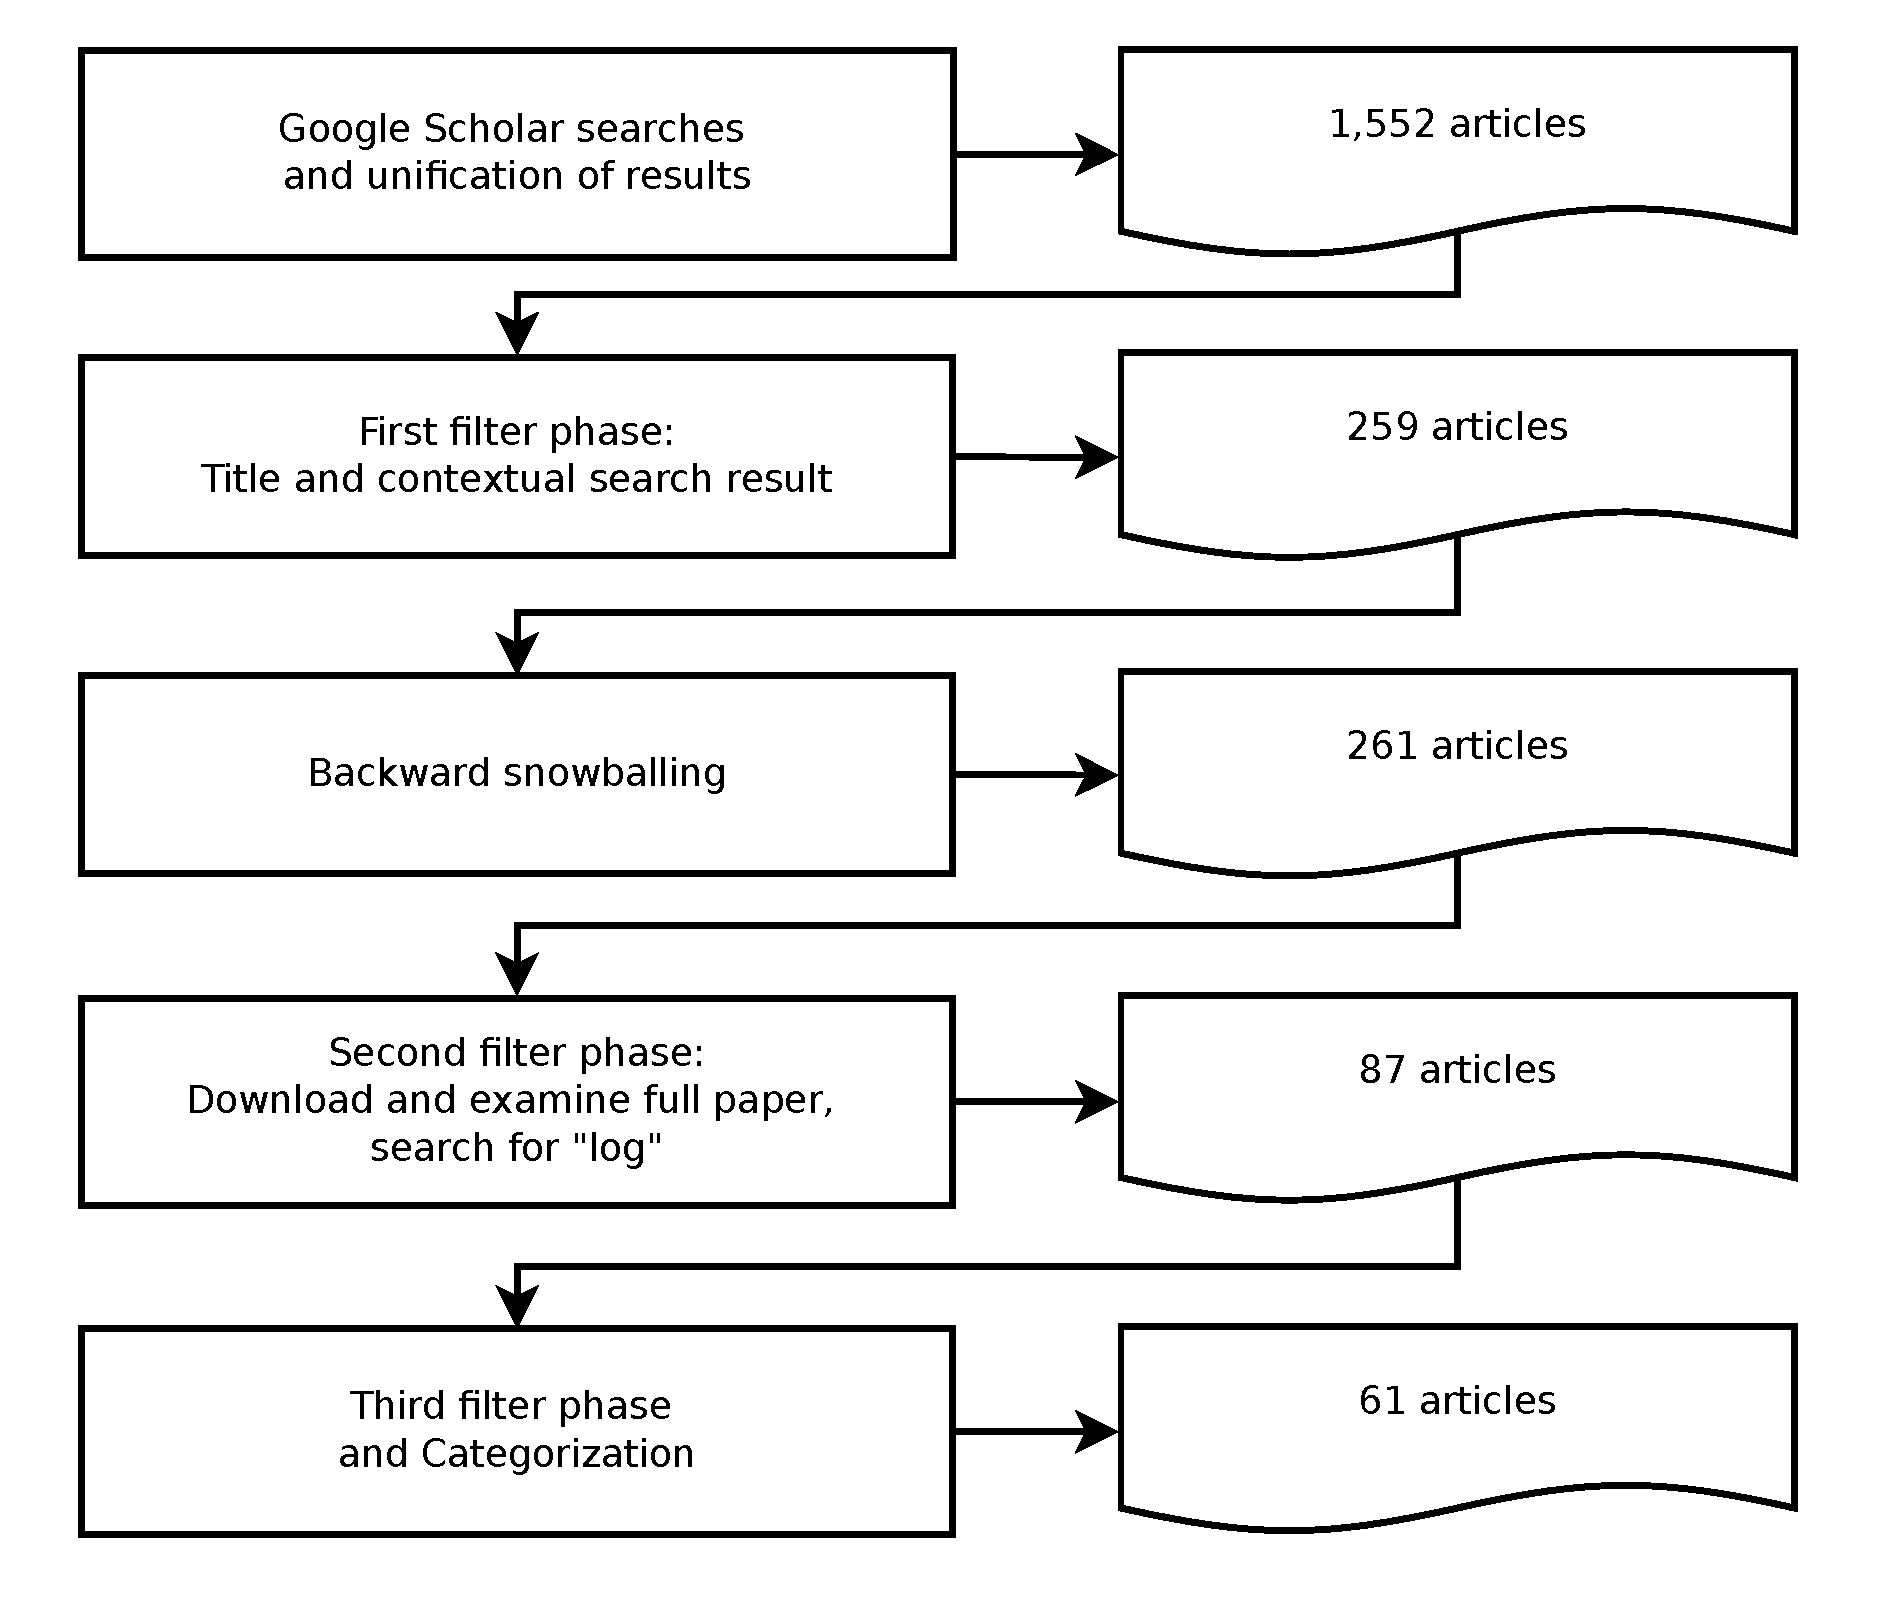
\includegraphics[width=\columnwidth, clip]{img/lit_survey.pdf}
	\caption{Our literature selection process, following
	\cite{petersen2015guidelines}.}
	\label{fig:lit-survey}
\end{figure}

The field of analyzing build
logs is relatively young; We have seen scattered
research efforts on build log analysis.
However,the processing of build logs was often
a side-part of the article.
To the best of our
knowledge, there has not been an attempt to systematically overview
and survey approaches for processing build logs.
We conducted a systematic mapping study to determine the
state-of-research on build log analysis following the guidelines
by Petersen et al.~\cite{petersen2008systematic,petersen2015guidelines}.

In the following section, we explain how build log analysis differs
from system log analysis.
Further, we describe how we selected the articles for our literature
survey and the data extraction from the resulting articles.
We present our results on how buildlogs are analyzed in literature
and discuss the implecations of these findings on our research.

\lstset{
  morekeywords={INFO, WARN, 2008, 11, 09},
  alsoletter=-20819,
  keywordstyle=\bfseries\color{Plum},
  escapeinside=**
}
\begin{figure*}[!tb]
  \centering
  \lstinputlisting[breaklines=true]{listings/syslog.txt}
  \caption{System Log excerpt.
Example adapted from~\cite{he2017towards}.}
  \label{lst:system-log}
\end{figure*}


\subsection{Distinction from System Log Analysis}
\label{sec:system-log-analysis}
A related field of build log analysis is the processing of system log
files produced during runtime.
A main difference between build logs
and system logs is that system logs are fundamentally structured
through events.
Each line in a log file represents one event with a
set of fields: timestamp, verbosity level and raw message
content~\cite{he2017towards}.
\Cref{lst:system-log} shows
example lines from a system log.

The first goal in analyzing system log files is ubiquitously to
separate constant and variable parts within a log
message~\cite{nagappan2010abstracting,he2017towards}.
Next, the log
messages are clustered into log events, unifying messages with
identical constant parts and varying parameters.
The output of a log
parser is an ordered list of timed events and their corresponding
parameter values~\cite{he2016evaluation}.
This structured log is then
the input to various machine learning and data mining processes.

The techniques developed for system log analysis can also be applied
to build logs.
One example is comparing execution traces to reference
traces of intended behavior to detect anomalies.
Amar et
al.~\cite{amar2019mining} employed a similar approach to detect
relevant lines in build logs.
However, many of the techniques developed to analyze system logs
leverage their inherent event structure.
As build logs lack this sturcture, we focussed our literature
survey on articles that as a source of information.
% In this article, we focus on extracting a single specified information
% from the build log as a whole with chunk retrieval techniques.
% Chunk
% retrieval techniques are used as a part of log parsing to retrieve the
% values of variable parts in a log message, e.g.\ by using regular
% expressions~\cite{nagappan2010abstracting,xu2009detecting}.


\subsection{Study Selection}
\Cref{fig:lit-survey} presents an overview of our study selection
process.
Since the field of build log analysis is so young, we
surveyed a population of scientific material as broad as possible.
We did not limit our sources to specific Software Engineering venues, as
is often done~\cite{petersen2015guidelines}, but survey all sources
monitored by Google Scholar, including Bachelor's and Master's
theses and academic slide decks.
We use Google Scholar as opposed to Scopus or
other databases, as it is the search engine for acdemic articles with
the broadest and most current index, including preprints.

Our Google Scholar search for variations of ``build log''
returns more than 2.2 million results (2020-03-15).
We refined our search criterions to exclude obvious
non-related works.
For example, we decided to exclude systems
or event logs (see \Cref{sec:system-log-analysis}).
This left us with 1,552 search results
(2020-03-15).
The full search queries are documented in our replication
package~\cite{brandt2020chunk-replication}.

To make handling so many search results feasible, we employed a
two-pass filtering strategy:

First, we filtered articles based on (1) their title and (2) the
contextual information Google Scholar displayed.
We inlcuded only
publications written in a language intelligible to the authors (that
is, English or German), which disregarded fewer than 1\% of search
hits.
We then unified
the results of the four search queries based on the link as the
identifying element, removing 60 articles that appeared in more than
one search query.
We removed further duplicates based on the title and were
left with 256 (16\%) of the original search results.
% removed duplicates of data extraction pass already here

With these 256 remaining articles, we followed a backward snowball
sampling for related work.
If one one of the articles referenced a new article in the context
of build log analysis we added the new to our literature set.
This added five papers (eight before
duplicate elimination), coming to a total of 261
articles.

Subsequently, we performed a second, finer filter phase by downloading the
full articles, reading their abstracts, and searching the full text
for the occurrence of ``log''.
If these papers showed traces of
working with build logs, we included them in our survey.
In total, we
were left with 87 articles after the two filtering phases.

\subsection{Article Classification}
Having trimmed down the set of articles, we investigated them in depth.

We wanted to characterize how researchers use buildlogs as input to
any processes.
We were interesed in
\begin{itemize}
  \item what information they are retrieving from the logs and
  what they use the retrieved information for (\textbf{RQ1.1})
  \item which technique they are using to process the build logs,
  in how much detail it is described and whether they published their
  tools (\textbf{RQ1.2})
  \item what kind of build logs they are using and the origin of these
  logs.
(\textbf{RQ1.3})
\end{itemize}
To objecifiy our data extraction we created a template of the targeted
factors and performed a pilot, as reccommended by Petersen et
al.~\cite{petersen2015guidelines}.
Two authors extracted the data from five articles and we held a
consensus meeting to unify our understanding
of the data extraction template.
The remaining articles were divided over these two authors.
We inspected the articles as closely as necessary,
starting from occurences of ``log'' or ``build'' within the text.

Relevant for our survey were all articles that
use logs from software builds as input to
some kind of process.
This excluded 15 articles from our study.
For several cases, multiple articles were extensions of others.
Of these, we only considered the earliest article which reported on
the processing of build logs.
This excluded another 11 articles.
In sum, we further extracted data from 61 articles.

The full data extraction template and our results of this step can be
found in our replication package~\cite{brandt2020chunk-replication}.
Note that for most questions we allowed assigning multiple values,
e.g.\ if
two kinds of information were targeted during a build log analysis.

\begin{simplebox}[attach boxed title to top center={yshift=-6mm}]
{\textbf{RQ1:} What is the state-of-research on build
log analysis?}
\begin{itemize}
  \item[\textbf{RQ1.1:}] Which information is targeted?
  \item[\textbf{RQ1.2:}] Which techniques are used?
  \item[\textbf{RQ1.3:}] Which build logs are analyzed?
\end{itemize}
\end{simplebox}

\subsection{Results}
In the following, we will present the results of our literature survey.
We present the information within the build logs that was targeted,
the retrieval techniques used and the origin of the build logs
which were analyzed.

\addtolength{\tabcolsep}{-5pt}
\begin{table*}[tbhp]
\tinyish
\centering
\caption{Overview of build log analysis techniques.}
\begin{tabularx}{\textwidth}{@{}lXl@{}}
\toprule
Name			     & Sources	& Frequency	  \\
\midrule
Parser	&
\cite{vassallo2018un-break,zhang2016android,seo2014programmers,hassan2019tackling,hassan2017automatic,chromy2007integration,mesbah2019deepdelta,wen2018blimp,kwon2018prioritizing,adams2007design,rahman2018impact,brandyberry2006continuous,tomassi2019bugswarm,ren2018automated,vassallo2019automated,cavalcanti2019impact,sippola2013qt,felipe2012towards,shi2018evaluating,urli2018design,selberg2012use}
&

\includegraphics[width=0.55\columnwidth]{img/lit-sur/techniques-no-guidelines-cropped_21.pdf}
\\
Regular expression
&\cite{beller2017oops,hassan2017change,macho2018automatically,vassallo2017a-tale,lou2019history,hassan2017automatic,rott2019empirische,zampetti2019study,zhao2018comparing,rausch2017empirical,ghaleb2019studying,zampetti2017open,zhang2019large,kavaler2019tool,morris2010experience}
&

\includegraphics[width=0.55\columnwidth]{img/lit-sur/techniques-no-guidelines-cropped_15.pdf}
\\
Manual inspection  &
\cite{sulir2016quantitative,hassan2017automatic,bouabana2019theory,barinov2017applying,silva2018build,ghaleb2019empirical,marcozzi2019systematic,hukkanen2015adopting,rausch2017empirical,hassan2017mining,zolfagharinia2017not,cassee2019impact}
&

\includegraphics[width=0.55\columnwidth]{img/lit-sur/techniques-no-guidelines-cropped_12.pdf}
\\
Machine Learning  &
\cite{hassan2017change,lou2019history,lindqvist2019detection,ren2018automated,schulz2017active}
&

\includegraphics[width=0.55\columnwidth]{img/lit-sur/techniques-no-guidelines-cropped_5.pdf}
\\
\makecell[cl]{Natural Language Processing}	&
\cite{hassan2017change,lou2019history,schulz2017active} &

\includegraphics[width=0.55\columnwidth]{img/lit-sur/techniques-no-guidelines-cropped_3.pdf}
\\
Information Retrieval  &
\cite{hassan2017change,lindqvist2019detection,ren2018automated} &

\includegraphics[width=0.55\columnwidth]{img/lit-sur/techniques-no-guidelines-cropped_3.pdf}
\\
Analysis  &
\cite{sulir2016quantitative,haghighatkhah2018test,durieux2019critical} &

\includegraphics[width=0.55\columnwidth]{img/lit-sur/techniques-no-guidelines-cropped_3.pdf}
\\
Keyword Search	&
\cite{brandyberry2006continuous,zhang2019large,kavaler2019tool} &

\includegraphics[width=0.55\columnwidth]{img/lit-sur/techniques-no-guidelines-cropped_3.pdf}
\\
Scan  & \cite{clemencic2014new,hibbard2001visualization} &

\includegraphics[width=0.55\columnwidth]{img/lit-sur/techniques-no-guidelines-cropped_2.pdf}
\\
Other  &
\cite{zhang2016android,hassan2017change,lou2019history,silva2018build,ren2018automated,schulz2017active}
&

\includegraphics[width=0.55\columnwidth]{img/lit-sur/techniques-no-guidelines-cropped_10.pdf}
\\
None identified  &
\cite{macho2017preventing,felipe2012towards,orellana2017differences,madeyski2017continuous,zhao2017impact,santolucito2018statically,makihara2018multi,mcintosh2012evolution,gallaba2018noise,matthies2016scrumlint}
&
\\
\bottomrule
\end{tabularx}
\label{tab:litsur:techniques}
\end{table*}
\addtolength{\tabcolsep}{5pt}
% TODO one source might contribute multiple times to 'other'

\begin{figure}
\centering
\begin{subfigure}[t]{\columnwidth}
		\centering
		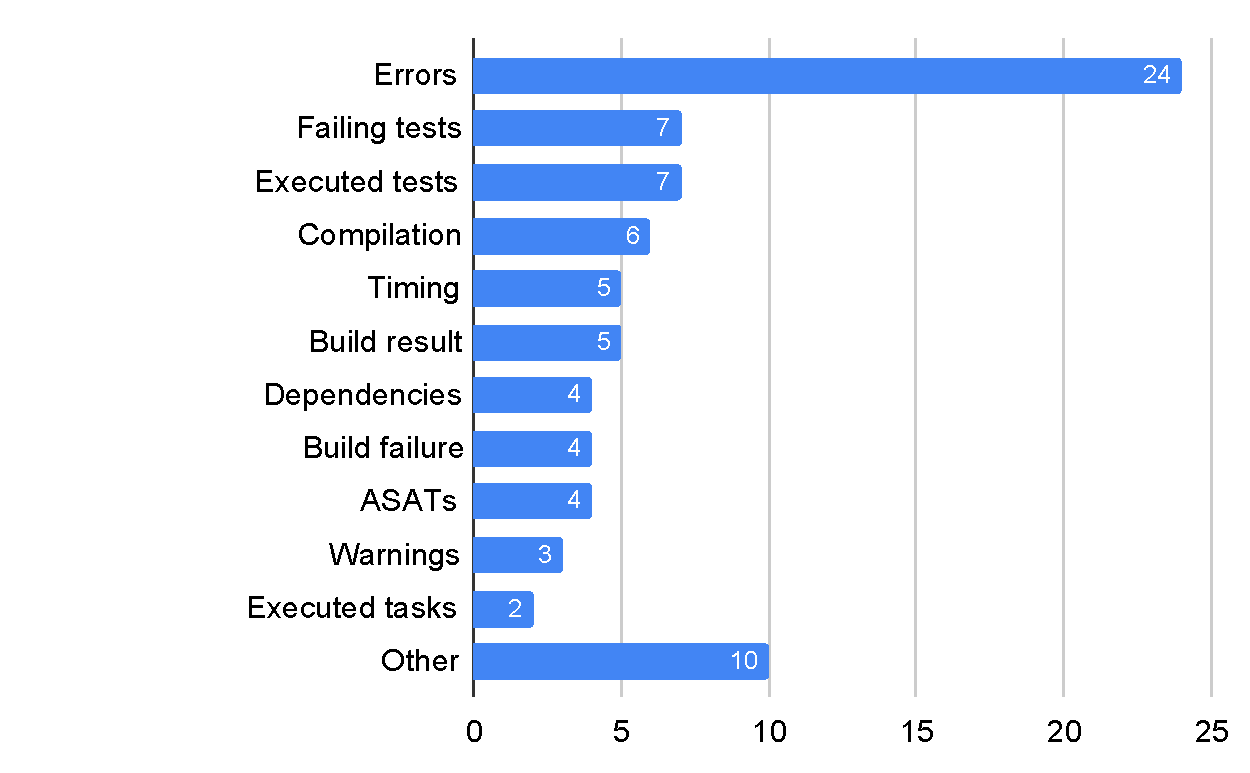
\includegraphics[width=\columnwidth,
		clip]{img/lit-sur/info_target.pdf}
		\caption{Information targeted in build log analysis.}
		\label{fig:litsur:info_target}

\end{subfigure}\hspace{\fill}
\begin{subfigure}[t]{\columnwidth}
		\centering
				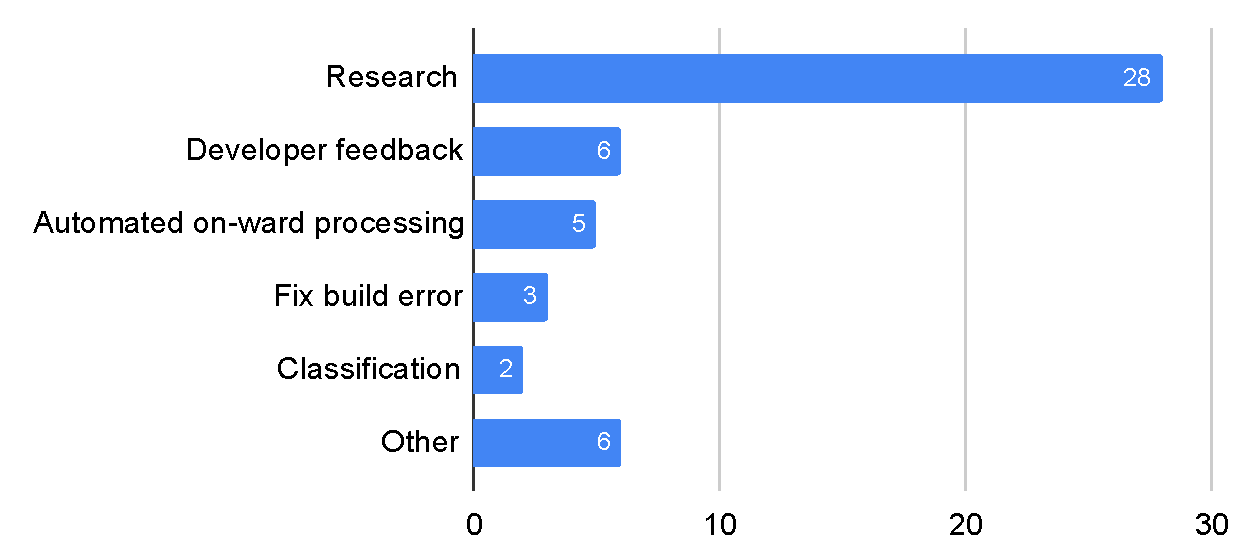
\includegraphics[width=\columnwidth,
				clip]{img/lit-sur/use.pdf}
		\caption{Purpose of build log analysis.}
		\label{fig:litsur:use}

\end{subfigure}

\caption{Multi-label categorization of the 61 relevant articles.}
\end{figure}

\begin{figure*}[tbhp]
		\centering
		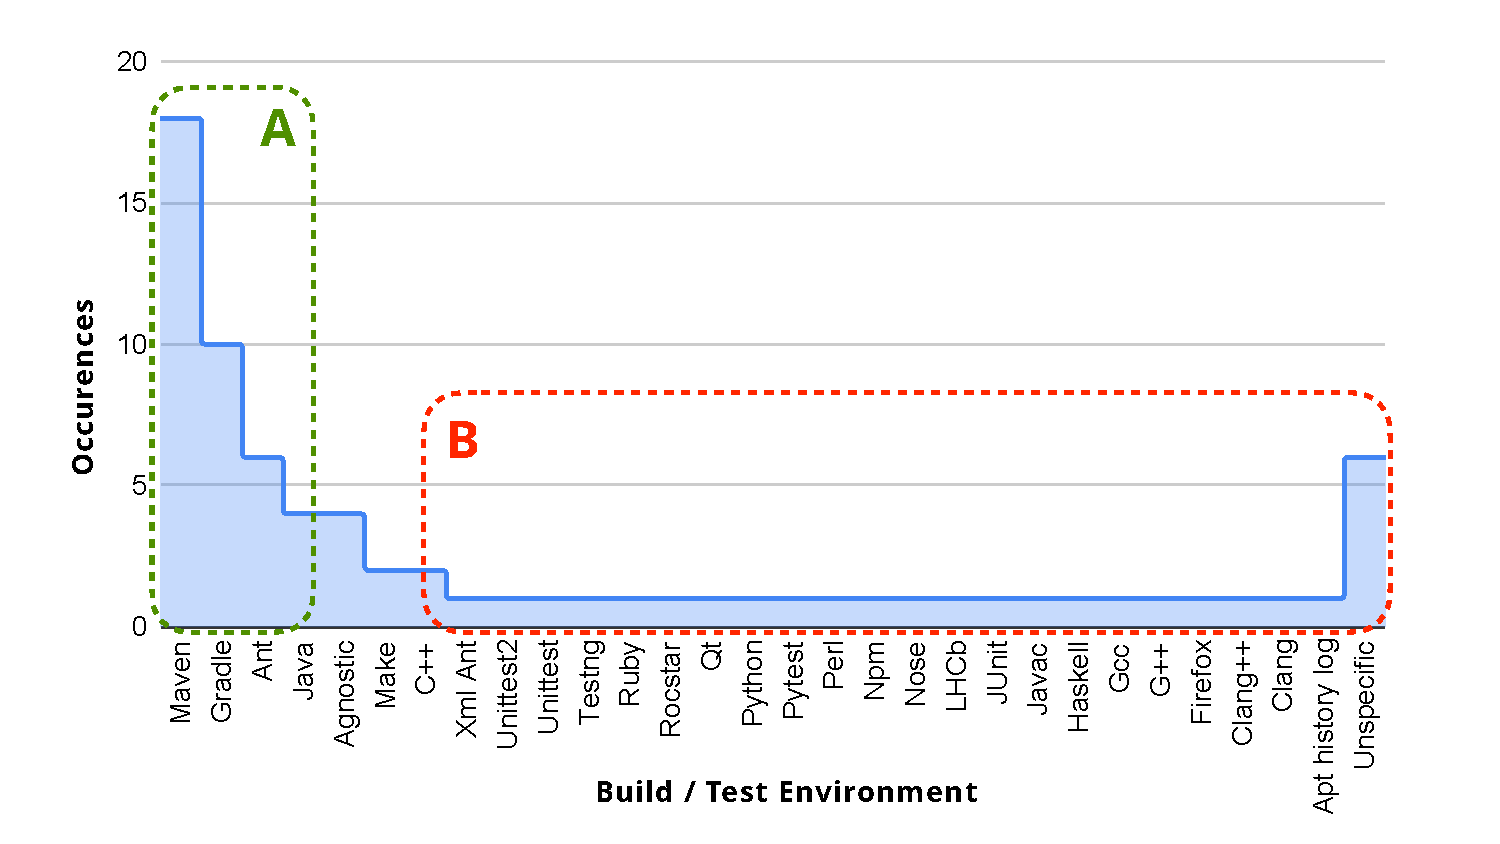
\includegraphics[width=0.7\textwidth, trim={1.1cm 0.4cm
		1.5cm 0.5cm},
		clip]{img/lit-sur/log_producer_annotated.pdf}
		\caption{Frequency of supported log producers.}
		\label{fig:litsur:log_producer}
\end{figure*}

\subsubsection{Retrieved Information}
The information that was targeted varied from article to article.
Most prominent was the search for errors (39\%) which occured within
the build process, as presented in \Cref{fig:litsur:info_target}.
This is followed by extracting the executed or the failing
tests (both 11\%).
There were also numerous cases which targeted more specialized
information, such as the environments used during the
build~\cite{zolfagharinia2017not}, packages
installed~\cite{selberg2012use} or hints to source files which are
related to build failures~\cite{ren2018automated}.

In most cases (51\%), a chunk was retrieved from the log.
Build logs were scanned for compilation
errors~\cite{clemencic2014new} or
the duration of tasks within the build~\cite{zhang2016android}.
36\% of the articles classified the build logs into categories.
For instance distinguishing failures caused by developers from
failures casued
by infrastructure errors~\cite{lindqvist2019detection} or
whether projects use automated statc analysis
tools~\cite{kavaler2019tool}.
Other types of information (e.g.\ counting
lines, summarization) were only retrieved
in one case each.

The majority of articles (46\%) used the outcome of their build log
analysis for research purpopses, as shown in \Cref{fig:litsur:use}.
Further uses were giving feedback to developers (10\%) or automatic
on-ward processing of the retrieved information (8\%).

\subsubsection{Retrieval Technique}
\Cref{tab:litsur:techniques} presents the techniques that the articles
described for processing build logs.
43 of the 61 articles we inspected mentioned how they are analyzing build
logs.
However, only 16 of these described their method in detail.

The most mentioned method (34\%) was using a parser, where we also
included
rather unprecise statements like ``we parse the build logs''.
25\% of the articles described the use of regular expressions and 20\%
inspected the logs manually.
Another 8\% employed machine learning techniques such as natural language
processing or information retrieval techniques.
To give examples,
Seo et al.~\cite{seo2014programmers} developed a custom
parser to classify error messages, while Vassallo et
al.~\cite{vassallo2017a-tale} analyzed build logs with regular
expressions.
Ghaleb et al.~\cite{ghaleb2019studying} used a compound approach.
They start with manual categorization of the build logs and select
search strings that identify their targeted categories.
Based on the search strings they create a script which automatically
classifies the remaining logs.

25\% of the articles claimed their implementation is available,
however we
saw very low reuse of build log analysis tools within our survey.
Five articles employed the tools used to create
\emph{TravisTorrent}~\cite{beller2017travistorrent,beller2017oops,
orellana2017differences,zhao2018comparing} or
an extended version of them~\cite{rott2019empirische,
shi2018evaluating},
two used the
\emph{Maven Log Analyzer}~\cite{macho2018automatically,gallaba2018noise},
another two the
\emph{MAKAO}~\cite{wen2018blimp,adams2007design,adams2007makao} tool.

% Seo et al.~\cite{seo2014programmers}
% They based their analyses on sets of
% build logs collected from industry partners.
% They	reported by Java and C++ builds.

% Rausch et al.~\cite{rausch2017empirical} analyze CI builds of open
% source Java projects

% Vassallo et al.~\cite{vassallo2017a-tale} compare open source projects
% in Java to industrial ones.
% Their data stems from analyzing
% build logs from \emph{TravisTorrent}~\cite{beller2017travistorrent}
% with regular expressions.

% Vassallo et
% al.~\cite{vassallo2018un-break}
% They parse
% Maven~\cite{maven2019website} build logs into a structured
% representation and create hint generators.
% For example, one of the hint generators queries stack overflow for
% discussions related to why the build failed.


\subsubsection{Build Logs}
The distribution of supported build tools is shown in
\Cref{fig:litsur:log_producer}.
Of the articles we surveyed, 30\% analyzed build logs produced by
Maven~\cite{maven2019website}, 16\% analyzed logs produced by
Gradle~\cite{gradle2020website}
and 10\% analyzed logs produced by Ant~\cite{ant2020website}.

Sometimes this limitation to a specific build tool is motivated by
aspects separate from the build log analysis.
For example, Shi et al.~\cite{shi2018evaluating} focussed on Maven
build logs because they also chose the PIT tool to calculate coverage
and mutation score.
A larger amount of the articles within our survey, however, limit
themselves to few build tools because their log format varies and
therefore ``parsers must be specialized to each build and test
framework''~\cite{tomassi2019bugswarm}.

Only 7\% of the proposed methods claimed to be language-agnostic, while
several described they are covering multiple source build tools.
The majority of articles (42\%) targeted logs from a source which was not
targeted by any second article.

The main platform that build logs were collected from is Travis
CI~\cite{travisci2019webpage},
which was used in 38\% of cases.
18\% of the articles processed logs from TravisTorrent and 8\% included
build logs from industrial projects.

The number of logs analyzed varied greatly and we were not always able to
extract it confidently.
Articles reported processing from two up to 122 million logs.

31\% of the surveyed articles claimed to have published their data to
enable further research.
However we found no clear reuse of build log data sets with the
exception of TravisTorrent~\cite{beller2017travistorrent}, which was
analyzed by Vassallo et al.~\cite{vassallo2017a-tale},
Ghaleb et al.~\cite{ghaleb2019studying} and several other studies.

\subsection{Discussion}
Our literature survey sheds light on how build log analysis is used within
computer science research.
In this section we will summarize our findings and relate them to the
approach we are taking to improve build log analysis with chunk
retrieval techniques.

We saw that various researchers process build logs to support their
research, often because the logs provide more or the necessary information
to the researchers~\cite{ren2018automated}.
Most of the articles which explicitly mention a manual analysis of
the logs only restrict their work to few logs or take a
``representative sample to make manual analysis
feasible''~\cite{zolfagharinia2017not}.
Automated approaches are necessary as many studies target a large
number of builds.
The chunk retrieval techniques we investigate within this article are
automated, apart from their configuration through training examples.

We have observed very little reuse of build log analysis tools.
This can stem from the fact that publishing replication packages and
research prototypes became popular only in recent years or from the
high specialization of the developed tools in regards to supported
build environments and targeted information.
Several articles noted the variety in log formats for different build
environments, which requires customizing build log techniques for
every supported build environment.
We implement build environment agonostic build log analysis
techniques, which are customized to a specific project by
the training examples which the user provides.
In addition, the \emph{LogChunks}~\cite{brandt2020logchunks}
data set we chose for our evaluation covers a broad range of build
environments.
Further, the training examples also specify the log chunk targeted by the
retrieval, which enable our chunk retrieval techniques to retrieve a
broad range of information from build logs.

Urli et al.~\cite{urli2018design} strongly discouraged from parsing
build logs for information as it is ``too error prone'', other
articles pointed to the effort of developing a custom tool.
Regular expressions are known to be tedious to
maintain~\cite{michael2019regexes}.
For this reason, we are focussing % TODO: less development time,
% only giving examples


This task of retrieving specific chunks of text from the
build logs can be solved by the chunk retrieval techniques we compare
in this article.
Our results can support researchers in choosing a
suitable technique for their data set of build logs and the chunks
they want to retrieve.
By relieving them from building custom parsers
we enable them to cover a much wider range of languages and build
tools in their studies.

% \subsubsection{Retrieved Information}
% why from build logs? not avaliable in cleaner format much use for
% research, a bit of developer information / tools following: research
% so many logs that unfeasible to do manually, less focus on tools for
% devs (caveat! we excluded books and documentation on industrial tools
% -> many approaches there to make build logs digestible, tough many
% focus on general minimizing of the data presented, not retrieving
% specific chunks)

% \subsubsection{Retrieval Technique}
% broadly mentioned shortly, rarely explained in detail we follow that
% researchers often see this as an unimportant side fact work needed to
% be done to get the big work done

% \subsubsection{Build Logs}
% often focussed on specific logs, sometimes mentioned because of effort
% developing a parser other times also because other tools used in
% further research are limiting the scope (reference paper with PIT
% tool).
% many focus on maven because of it's prevalence also in respect
% to other tools much research done on travis ci logs b/c of their
% abundance and open availability
\section{Chunk Retrieval Techniques}
\label{sec:techniques}
This section introduces key concepts of the three chunk retrieval
techniques we study in this article, namely program synthesis by
example (PBE), common text similarity (CTS), and keyword search (KWS).

\Cref{tab:ctr} shows a comparison of the presented techniques.

\subsection{Characteristics of Chunk Retrieval Techniques}
\label{sec:blirt}
In this article, we evaluate different techniques to automatically
retrieve pieces of information that appear literally in the build
logs.
%, i.e., techniques that do not aggreagte, combine, or deducted
%information.
We call such pieces of information from build logs
\emph{chunks}, and the techniques \emph{chunk retrieval techniques}.
The techniques we investigate here do not require a formal lexer and
parser to analyze the entire structure of build logs, but focus on
ad-hoc extracting just one specific piece of information per
configuration.

With the term \textit{configuration}, we abstract over the training
and parametrization that different techniques require in different
forms.
A configuration can be explicitly stated or implicitly dervied
by learning through provided examples.
It is therefore a manual
specification of which information the chunk retrieval should target.
It also supplies the necessary information for the technique to
identify the targeted information chunk in a build log.
Each chunk
retrieval technqiue has a specific \textit{granularity}, i.e.,\ the
smallest piece of text it can return (e.g., a line, or a word).
The
granularity might be adjustable by configuration.
\emph{Running a
chunk retrieval technique} means to execute a fully configured
technique to consumes as input a build log in plain text format and to
produce an array as output.
The array consists of substrings of the
build log text.


\begin{table*}[]
\centering
\caption{Chunk retrieval techniques.}
\begin{tabularx}{\textwidth}{@{}XlXlXX@{}}
\toprule
Name			     & Acronym & Identification Technique
& Granularity & Configuration & Source		  \\
\midrule
Program Synthesis by Example & PBE     & Regular expression program
& Character   & In/output examples	\\
Common Text Similarity	     & CTS     & TF-IDF \& cosine similarity,
expected number of lines & Line        & Output examples	   \\
Keyword Search		     & KWS     & Keywords, expected number of
lines			 & Line        & Keywords, context length  \\
Random Line Retrieval	     & RLR     & Random sample
& Line	      & Retrieval length	  \\
\bottomrule
\end{tabularx}
\label{tab:ctr}
\end{table*}


\subsection{Program Synthesis by Example (PBE)}
\label{sec:expl-pbe}
The concept of \emph{Programming by Example} aims to capture the
intent of the user through examples which they provide.
Leveraging this apprach, we implemented a chunk retrieval technique
for build logs.
Our implementation is based and highly influenced by the
\emph{Microsoft PROSE library}~\cite{prose2019webpage}.
The PROSE library is powered by the generic program synthesis framework
\emph{FlashMeta}~\cite{polozov2015flashmeta:} and the specialized
text extraction DSL \emph{FlashExtract}~\cite{le2014flashextract:}.
Both enable us to synthesize regular expression programs
consistent~\cite{mitchell1982generalization} with a set of in-
and output examples given by the user.
The usage of example enables the user to configure a chunk
retrieval without understanding the whole structure of
the build log.

\subsubsection{Configuration}
In- and output example pairs are the main driver of Programming by
Example, we refer to them in short as \emph{examples}.
The \emph{input} is the text of the build log file.
The \emph{output} is
a substring of the log file text, representing the
substring that should be retrieved by the synthesized program when
given the corresponding input file.
One or multiple examples, the
training set, \emph{configure} a specific chunk retrieval with PBE:
they define the substring of a build log that should be extracted.
The PROSE program synthesis then tries to construct a program
consistent with all training examples.
If PROSE cannot synthesize a program, e.g.\
because the regular expression
necessary would be too complicated to synthesize, PBE returns the
error message ``no program found''.
\Cref{lst:prose-program-simplified} presents a simplified version
of a program learned from the examples in \Cref{lst:chunk-example}.
% TODO Caro: check that these figures are latest inserted here


% TODO Moritz: you said: The following is very obvious and could apply
% to any
% % technique.
% % kinda.
% It does give a descriptive error message on no match (and
% % that is not possible in other techniques)
% % otherwise yes, nothing interesting happens in the application of pbe
% % though for consistency we might need this section? or merge
% config/application?
\subsubsection{Application}
A run of PBE takes a build log file as input and applies the
synthesized regular expression program.
It then returns the substring
of the build log matched by the program or an error message if the
program found no match.


\subsection{Common Text Similarity (CTS)}
\label{sec:expl-ts}
Text Similarity approaches are widely used to filter unstructured
textual software artifacts~\cite{runeson2007detection,
marcus2005recovery,antoniol2002recovering,mccarey2006recommending}.
We investigate a chunk retrieval technique based on the common
Vector Space Model~\cite{schutze2008introduction}.
The aim is to retrieve those lines from a build log which are most
similar to examples given by the user.

\subsubsection{Configuration}
To configure chunk retrieval though text similarity we chose to use
the same concept of examples as for PBE
% TODO Moritz: your question was: More details on this.
% How do you
% 'apply' VSM? On what?
% all the following sentences in this subsubsection describe our way
% of determining text similarity which as far as I understand and
% Annibale said is the VSM.
% word tokens, tf-idf, similarity measure
% I added a "as follows", think that is enough for explanation?
and apply the Vector Space Model~\cite{schutze2008introduction}
as follows:
The lines of the output strings of the training examples define our
search query.
The algorithm splits the search query into single lines and
identifies tokens, in our case words.
Then we build a
document-term-frequency matrix over the lines from the search query
and prune very often or very rarely appearing words.
Finally, the
algorithm applies TF-IDF to the matrix, a best practice for natural
language queries~\cite{lee1997document}.

\subsubsection{Application}
To retrieve the desired information from a build log, we parse the
whole text and process it in the same way as the search query.
The algorithm calculates the cosine
similarity~\cite{korenius2007principal} to compare each line of the
build log with each line of the search query.
After summing up the
similarities of each build log line to all search query lines, we sort
the build log lines in decreasing similarity.
The average number of
lines in the outputs of the training examples determines how many of
the most similar lines are returned as the output of the retrieval
run.

\subsection{Keyword Search (KWS)}
\label{sec:expl-skws}
When developers scavenge for a specific piece of information within a
large amount of unstructured information, a first ad-hoc approach they
use is to search for related keywords.
Indeed, this was one of the
most common approaches we took when searching for the reason a build
failed while creating the \emph{LogChunks} data
set~\cite{brandt2020logchunks}.

\subsubsection{Configuration}
A set of keywords configures the chunk retrieval with KWS\@.
To better
compare KWS with PBE and CTS, we also configure it through examples.
We associate each example with keywords which appear in the targeted
chunk or close to it.

KWS then searches for those keywords which are tied to the greatest
number of examples in the training set.
If several keywords are associated with the same number of training
examples, and no other keywords are associated with more training
examples, KWS searches for all of these keywords.

\subsubsection{Application}
For a retrieval run, we take a whole build log file as input and
search for all exact occurrences of the keywords.
As keywords are
often not directly describing the desired information, but rather
appear close to the desired information, KWS also retrieves the lines
around the found keyword.
The number of surrounding lines retrieved is
the average of lines in the output of the training examples.


\subsection{Random Line Retrieval}
\label{sec:expl-rlr}
In our evaluation, we want to compare against a baseline of randomly
picking lines from the build log.
RLR mimicks the
situation of guessing blindly which lines might be interesting.
The only configuration option for RLR is the number of lines it should
return.
For a fair comparison to the other techniques (whose number of
returned lines is dynamic), we configure RLR to return the average
number of lines in the chunks of the training examples.

% TODO Moritz: you said: some more details here?
% I would not know of any details to add.
%It's really all we are doing

\subsection{Tool Implementation}
For our comparison study we implemented each of the chunk retrieval
techniques and a unifying interface.
The unified interface is implemented in Ruby and
calls the separate technique implementations over the command line.
The implementation of PBE in C\# is based on the Microsoft PROSE
library~\cite{prose2019webpage}.
We implemented CTS, KWS and RLR using
R and the text2vec library~\cite{text2vec2019webpage}.


\section{Study Design}
\label{sec:study}

\begin{simplebox}[minipage boxed title*=-2.5cm,
attach boxed title to top center={yshift=-6mm}]
{\textbf{RQ2:} When are PBE{,} CTS or KWS suited to
retrieve chunks from build logs?}
\begin{itemize}
  \item[\textbf{RQ2.1:}] How many examples does a technique need to
  perform best?
  \item[\textbf{RQ2.2:}] How structurally similar do the examples
  need for a technique to be applicable?
  \item[\textbf{RQ2.3:}] How accurate are the retrievals of a technique?
\end{itemize}
\end{simplebox}

% TODO Caro: redo
\begin{figure*}[tb]
	\centering
	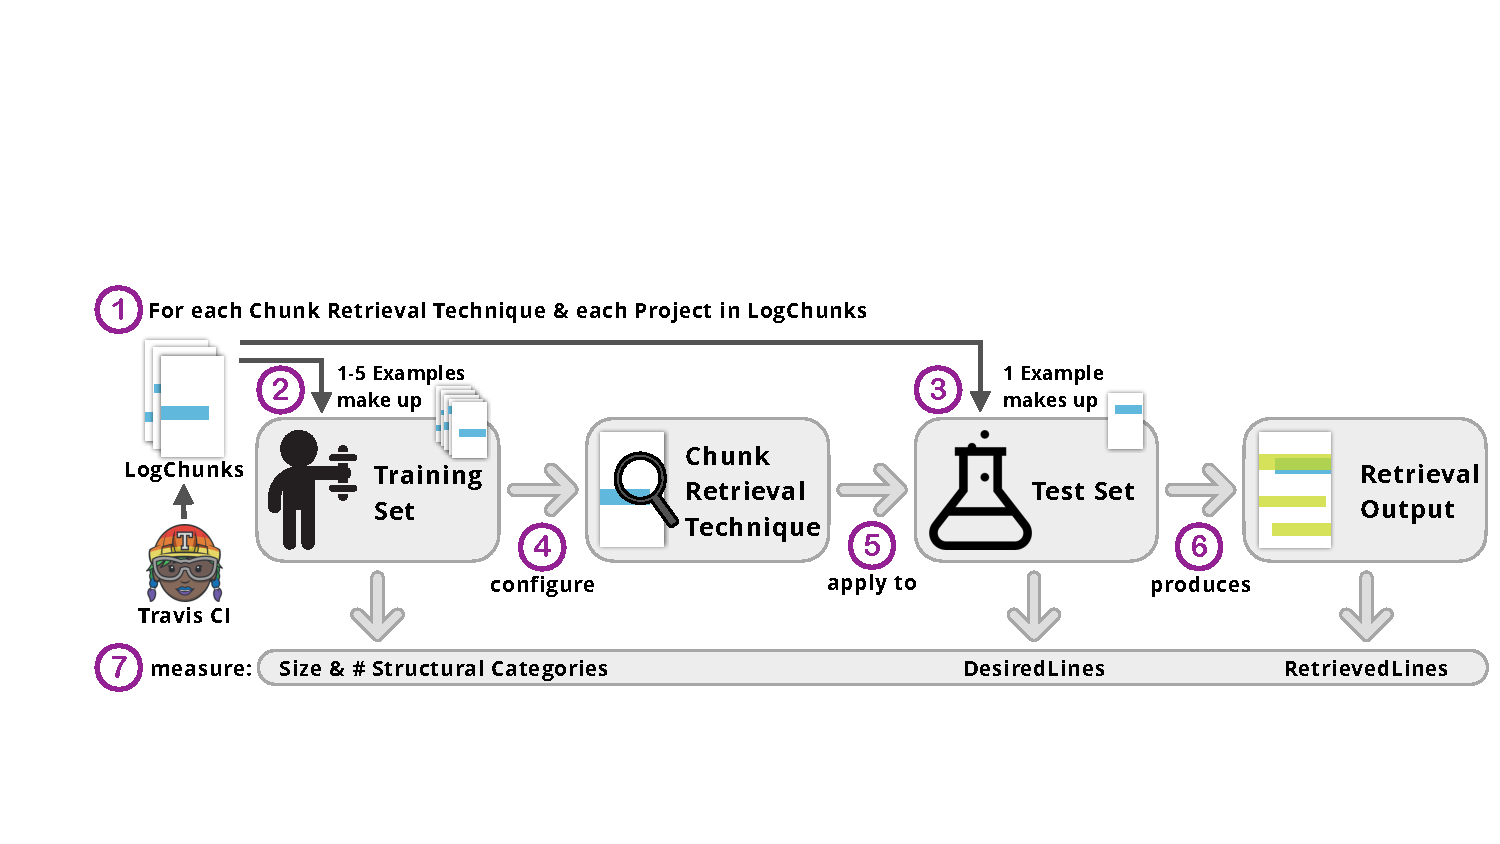
\includegraphics[width=\textwidth, trim={1.6cm 1.6cm 0.2cm 5.6cm},
  clip]{img/study.pdf}
	\caption{Design of our technique comparison study.}
	\label{fig:study}
\end{figure*}

To investigate which technique is best suited to retrieve chunks from
CI build logs we evaluate the three chunk retrieval techniques
PBE, CTS and KWS.
Random Line Retrieval (RLR), acts as a baseline for
the comparison.
The following section
describes our study design and which metrics we measure to answer our
research questions.
In the presentation of the results, we first focus
on each of the three techniques and later compare them against each
other.

\subsection{LogChunks}
For this study we created the previously published data set
\emph{LogChunks}.
It encompasses 797 build logs from Travis CI,
stemming from a broad range of 80 GitHub repositories and 29
programming languages.
For each file, the authors manually ``labeled
the log part (chunk) describing why the build
failed''~\cite{brandt2020logchunks}.
We include keywords, which we
would use to search for the selected chunk within the log.
In
addition, we categorized the log chunks according to their format
within the log.
If the chunks are surrounded by the same markings
within the log we assign them the same structural category.

% We run four techniques on the examples from \emph{LogChunks}.

\noindent
\textbf{Training and Test Set}
% TODO Moritz: You said: Add details how key words were extracted.
% Add example?
% how the keywords were put in logchunks does not fit here, that is
% maybe answered 2 paragraphs above already?
% how KWS uses the keywords is already described in the section
% introducing the technique => I would scrap everything but the first
% sentence directly above here :)

% TODO Moritz: You said: Add more details.
% How was the split in numbers?
% this is described in the following paragraph, should we merge them
% (bc there are also no sub-RQs now) or is it close enough? :)
For each repository in \emph{LogChunks}, we split the examples
chronologically into training and test set.
Therefore, we train on
examples from past build logs and test on more recent build logs.

\noindent % TODO: adapt if we change the research questions
\textbf{RQ 2.1: Size of Training and Test Set}
We evaluate the techniques with different training set
sizes, to analyze how many examples the chunk retrieval techniques need to
perform best.
We train each technique with one to five examples from each of
the repositories within \emph{LogChunks}.
The size of the test set is one.

\noindent
\textbf{RQ 2.2: Recording Structural Categories}
We record the structural categories
of the examples in the training and test sets, to determine how
structurally similar the examples for the chunk
retrieval techniques need to be.

\noindent
\textbf{RQ2.3: Accuracy Metrics}
we save the output lines of the chunk retrieval run on the input
of the test example ($\mathit{RetrievedLines}$), to measure the
accuracy of the retrieved chunks
As oracle in our evaluation, we save the
desired lines from the output of the test example
($\mathit{DesiredLines}$).

We calculate and define a number of metrics for the context of our
evaluation.

\vspace{0.2cm}
\begin{itemize}[leftmargin=0.4cm] \itemsep1em
	\item $|\mbox{True\ Positives}| = \mathit{DesiredLines} \cap
	\mathit{RetrievedLines}$ \vspace{0.2cm}\\
	True positives are lines that appear both in the output of a
	tool as well as what \textit{LogChunks} contains for the
  test example.

	% What about when a line is replicated twice?
	% I.e., Are line numbers part of this? => no.
	% not checked, but if lines are identical they also contain
	% the same information so if someone asks we can defend I think
	\item $\mbox{Precision} = \dfrac{|\mathit{True\
	Positives}|}{|\mathit{RetrievedLines}|}$ \vspace{0.21cm} \\
	Precision of a chunk retrieval describes which proportion of
	the retrieved lines were actually desired.

	\item $\mbox{Recall} =
	\dfrac{|\mathit{True\ Positives}|}{|\mathit{DesiredLines}|}$
	\vspace{0.2cm} \\
	Recall of a chunk retrieval describes which proportion of the
	desired lines were retrieved.
	\item $\mbox{F$_{1}$-score} = 2 \cdot \dfrac{\mathit{Precision}
	\cdot \mathit{Recall}}{\mathit{Precision} + \mathit{Recall}}$
	\vspace{0.2cm}\\
	In addition, we calculate the F$_{1}$-score, the harmonic mean
	of precision and recall.
We prefer F$_{1}$ to other aggregate
	measures such as accuracy because for a
	``needle-in-the-haystack'' scenario, we do not want to bloat
	our results by correctly not finding lots of irrelevant log
	lines.
	\item Successful retrieval = $\mathit{true}\ \mathit{iff}\
	\mathit{Recall} = 1, \mathit{false\ otherwise}$  \vspace{0.2cm} \\
	We define a successful retrieval as one where all desired
	lines were
	extracted, therefore when recall is one.
\end{itemize}


\section{Results}
This section presents the separate results for each chunk retrieval
technique.
Afterwards we compare the three techniques with each other and RLR as
baseline.



\subsection{Program Synthesis by Example (PBE)}
\label{sec:r:pbe}

\begin{figure}[tbp]
		\centering
		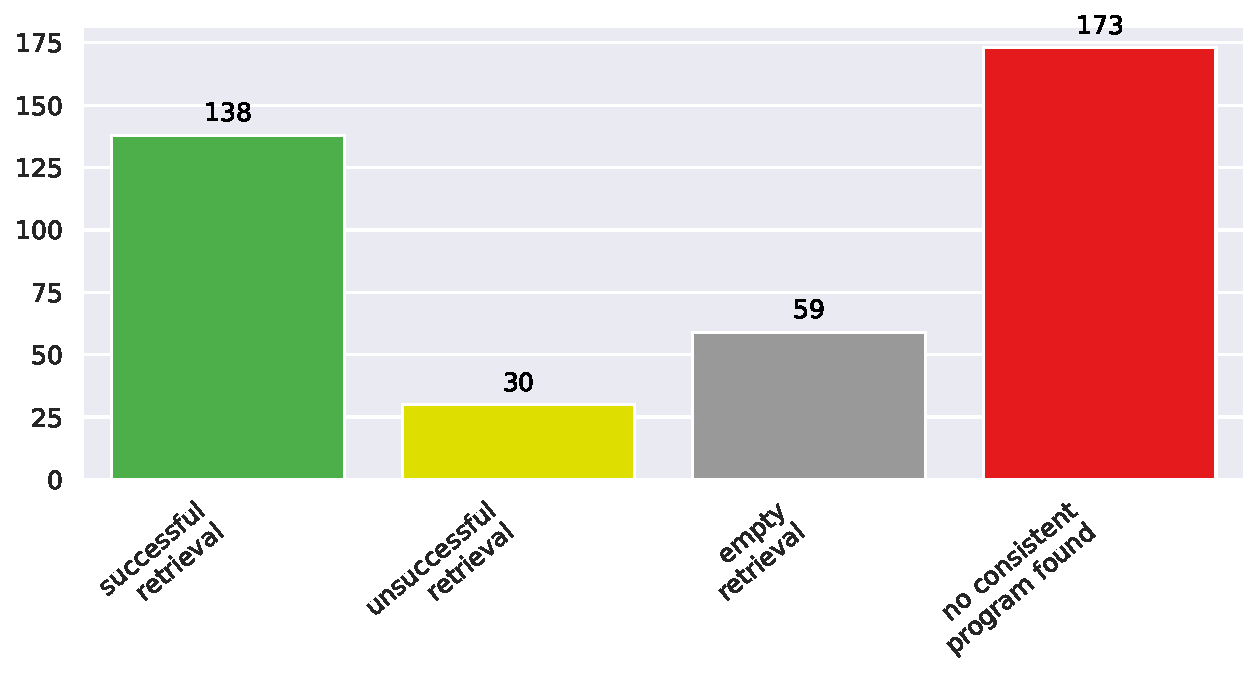
\includegraphics[width=\columnwidth,
		clip]{img/big-study/failure-reason-pbe.pdf}
		\caption{Results of chunk retrieval with PBE.}
		\label{fig:failure-reason-PBE}
\end{figure}

\lstset{
  language=,
  morekeywords={Test, Output, Desired},
  keywordstyle=\textbf,
	frame=single
}
\begin{figure}[!t]
  \centering
  \begin{lstlisting}[breaklines=true]
Test Output:
Error: Invalid CSS after "2.3em": expected expression (e.g.
1px, bold), was ";"
	on line 86 of sass/components/dropdown.sass
Desired Test Output:
Error: Invalid CSS after "2.3em": expected expression (e.g.
1px, bold), was ";"
	on line 86 of sass/components/dropdown.sass
	from line 5 of sass/components/_all.sass
	from line 6 of bulma.sass
  \end{lstlisting}
  \caption{Example for an unsuccessful retrieval (PBE retrieved only
  two of the four targeted lines).}
  \label{lst:pbe-unsuccessful}
\end{figure}

\begin{figure*}
\centering
    \textbf{Program Synthesis by Example (PBE)}\par\medskip
\begin{subfigure}[b]{\columnwidth}
		\centering
		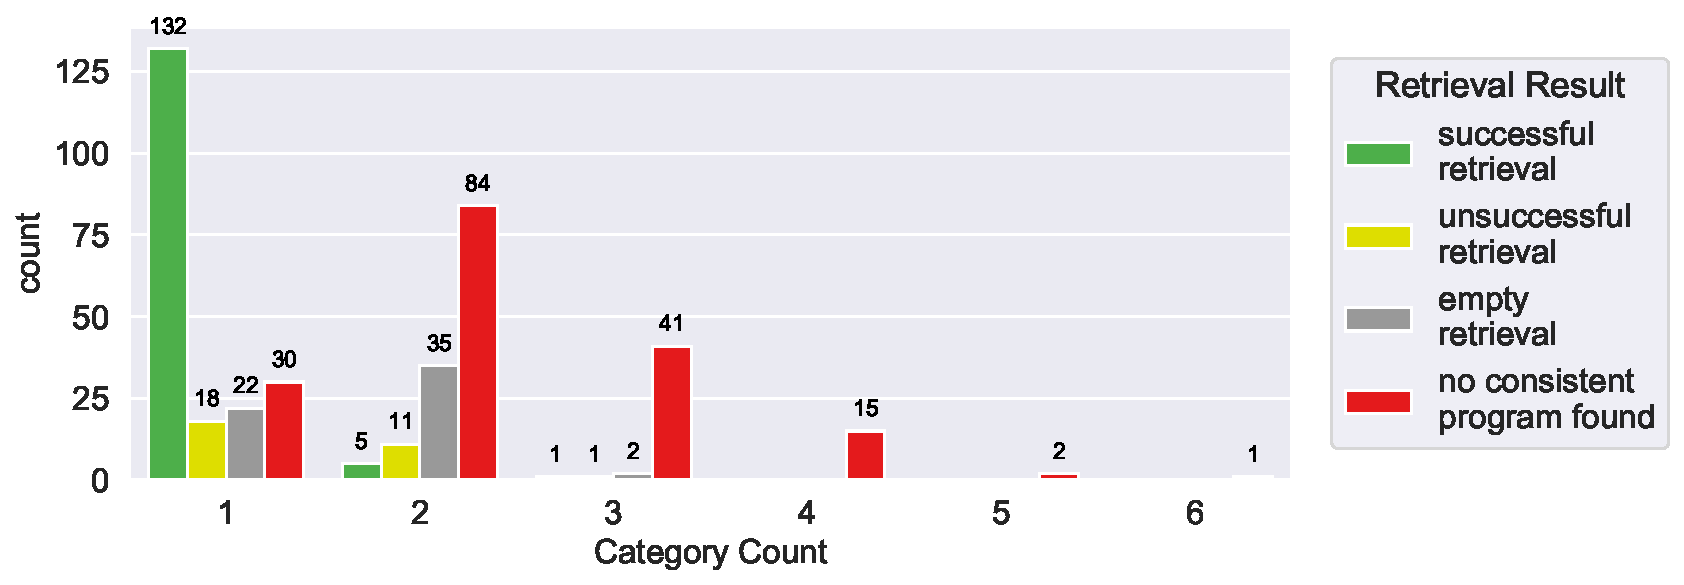
\includegraphics[width=\columnwidth,
		clip]{img/big-study/failure-reason-categorycount-PBE.pdf}
				\caption{Successfulness of retrieval
				compared by structural category count
				in training and test sets.}
		\label{fig:failure-reason-categorycount-PBE}
\end{subfigure}\hspace{\fill}
\begin{subfigure}[b]{\columnwidth}
		\centering
		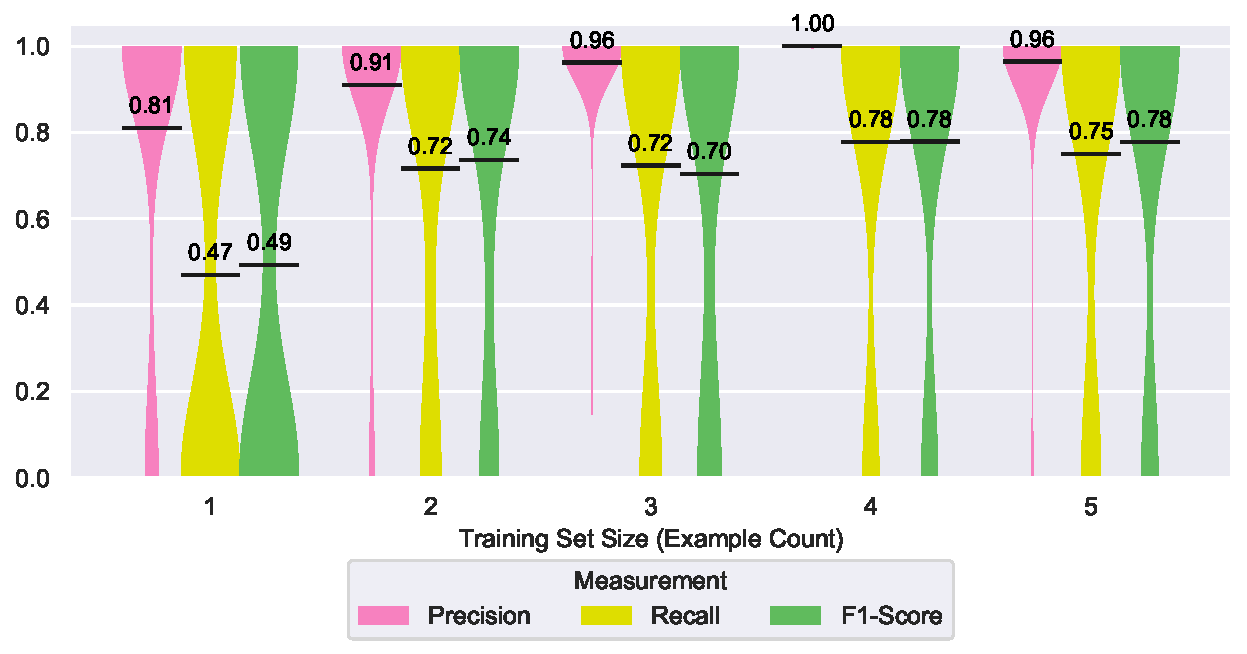
\includegraphics[width=\columnwidth,
		clip]{img/big-study/recall-precision-examplecount-sythesisworked-PBE.pdf}
				\caption{Precision, recall and
				F$_{1}$-score when PBE could synthesize
				a consistent program compared with the
				size of the training set.}
		\label{fig:recall-precision-examplecount-sythesisworked-PBE}
\end{subfigure}
\caption{Results of chunk retrieval with  Program Synthesis by Example
(PBE)}
\end{figure*}

\Cref{fig:failure-reason-PBE} presents the results of the chunk
retrieval with PBE.
Out of the 400 runs, 5 per each one of the 80 example
sets, PBE extracted all the desired lines successfully in 138 cases.
In 59 cases, a regular expression program could be synthesized, though
it did not find a match on the test build log.
In 30 cases the synthesized program only extracted a
subset of the desired lines.
For these 30 cases, the average recall
was 28\%.
\Cref{lst:pbe-unsuccessful} shows how an example of such
an \emph{unsuccessful retrieval}, where the synthesized program only
retrieved two of the four targeted lines.
In 173 of the 400 cases
could PROSE not synthesize program consistent with all of the training
examples.

\Cref{fig:failure-reason-categorycount-PBE} shows the results of PBE
runs depend on the number of structural categories in the training and
test examples.
The figure demonstrates that program synthesis mostly
returns exactly the desired output when there are is only one
structural category present in the training and test examples.
However, when
two or more structural categories are simultaneously present,
PROSE could in most cases not synthesize a program.
For four or more present
categories PROSE could never synthesize a consistent program.

\Cref{fig:recall-precision-examplecount-sythesisworked-PBE} shows
precision and recall of the 227 runs where PBE could synthesize a
program consistent with all training examples.
When the training set
size increases from one to two, recall and F$_{1}$-score increase by
about 25\%, precision increases by about 10\%.
For two or more
training examples, recall and F$_{1}$-score stay around 75\% and
precision around 96\%.

\subsection{Common Text Similarity (CTS)}
\label{sec:r:cts}
\begin{figure*}
\centering
    \textbf{Common Text Similarity (CTS)}\par\medskip
\begin{subfigure}[tb]{\columnwidth}
		\centering
		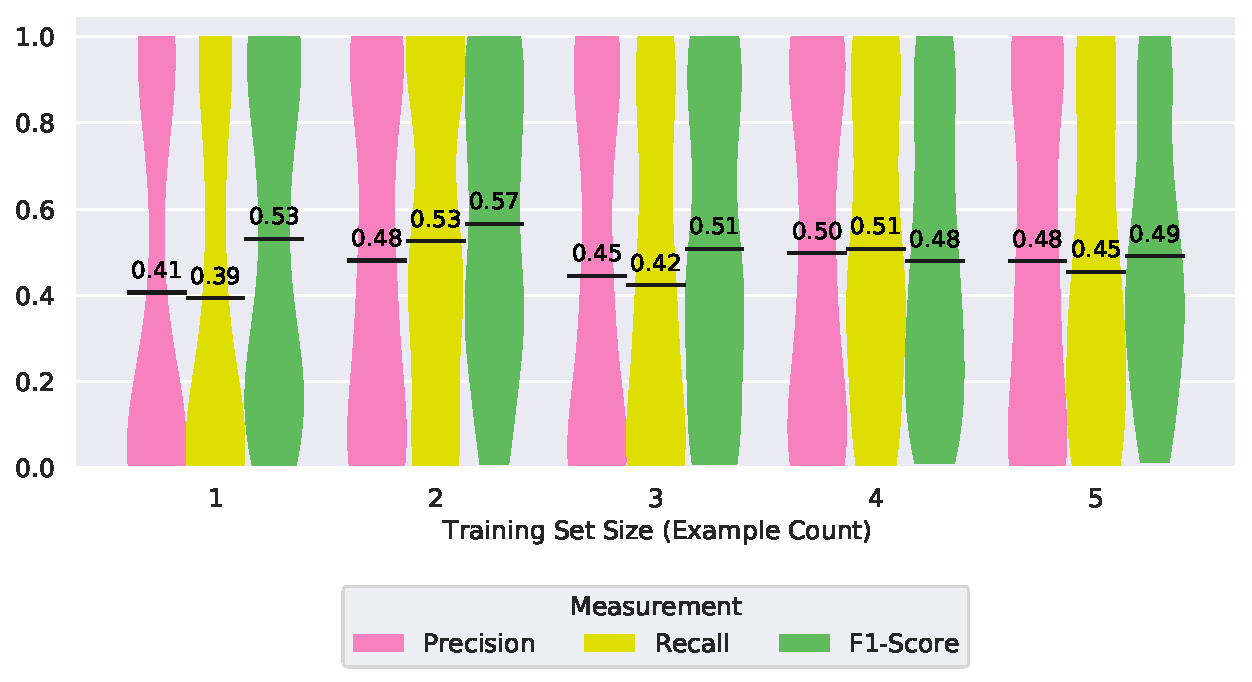
\includegraphics[width=\columnwidth,
		clip]{img/big-study/recall-precision-examplecount-CTS.pdf}
		\caption{training set size.}
		\label{fig:recall-precision-examplecount-CTS}

\end{subfigure}\hspace{\fill}
\begin{subfigure}[tb]{\columnwidth}
		\centering
				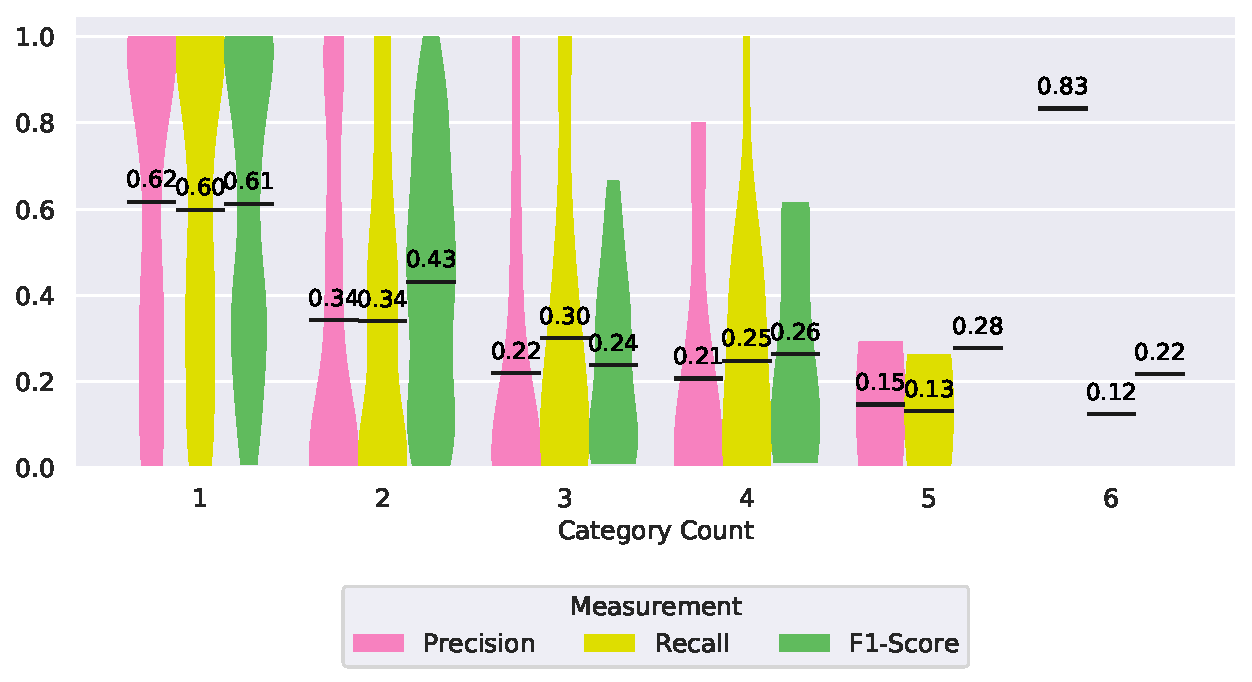
\includegraphics[width=\columnwidth,
				clip]{img/big-study/recall-precision-categorycount-CTS.pdf}
		\caption{structural category count
		in training and test set.}
		\label{fig:recall-precision-categorycount-CTS}
\end{subfigure}
\caption{Precision, recall and F$_{1}$-score of chunk
retrieval with Common Text Similarity (CTS) compared by \ldots}
\end{figure*}

\Cref{fig:recall-precision-examplecount-CTS} presents precision,
recall and F$_{1}$-score of chunk retrieval using CTS for an
increasing number of training examples.
When using one to five
training examples, the size of the training set has no noticeable
influence on precision, recall or F$_{1}$-score of the chunk retrieval
with CTS.

\Cref{fig:recall-precision-categorycount-CTS} shows the same
measurements for an increasing number of structural categories in the
training and test examples.
With increasing category count, precision,
recall and F$_{1}$-score decrease.
% Especially for more than four
% categories present we have no chunk retrieval runs where all desired
% lines were extracted.

\subsection{Keyword Search (KWS)}
\label{sec:r:kws}
\begin{figure*}
\centering
    \textbf{Keyword Search (KWS)}\par\medskip
\begin{subfigure}[b]{\columnwidth}
		\centering
		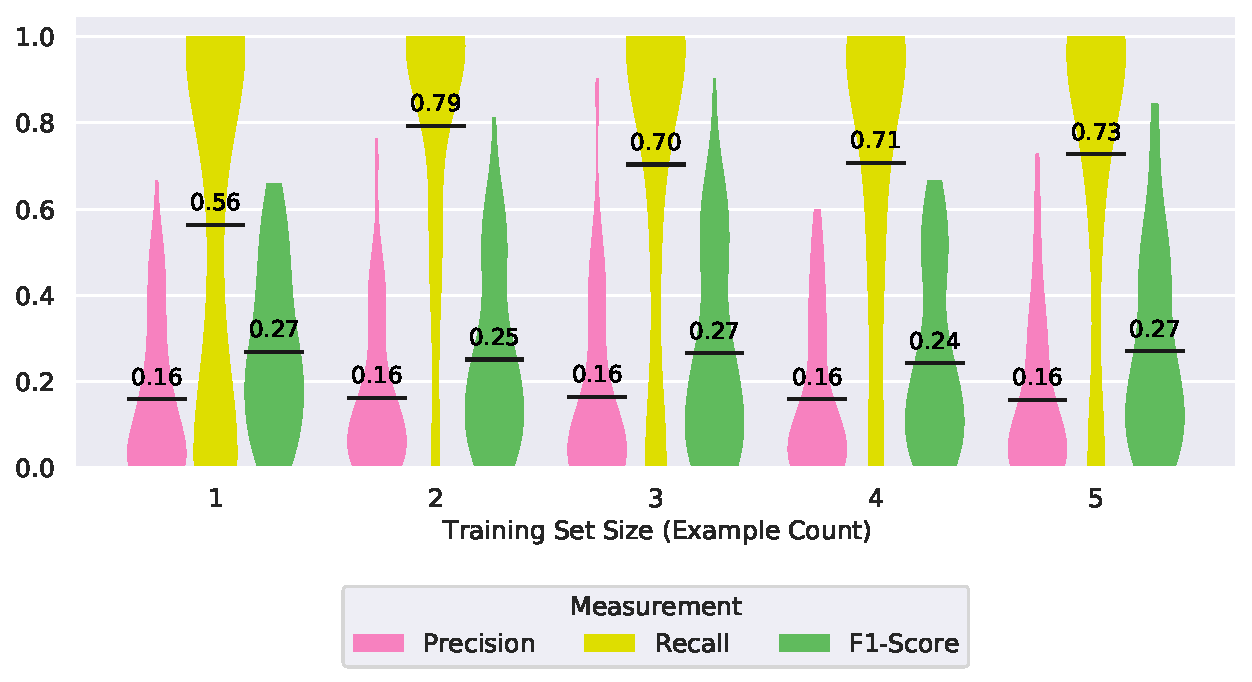
\includegraphics[width=\columnwidth,
		clip]{img/big-study/recall-precision-examplecount-KWS.pdf}
		\caption{training set size.}
		\label{fig:recall-precision-examplecount-KWS}
\end{subfigure}\hspace{\fill}
\begin{subfigure}[b]{\columnwidth}
		\centering
		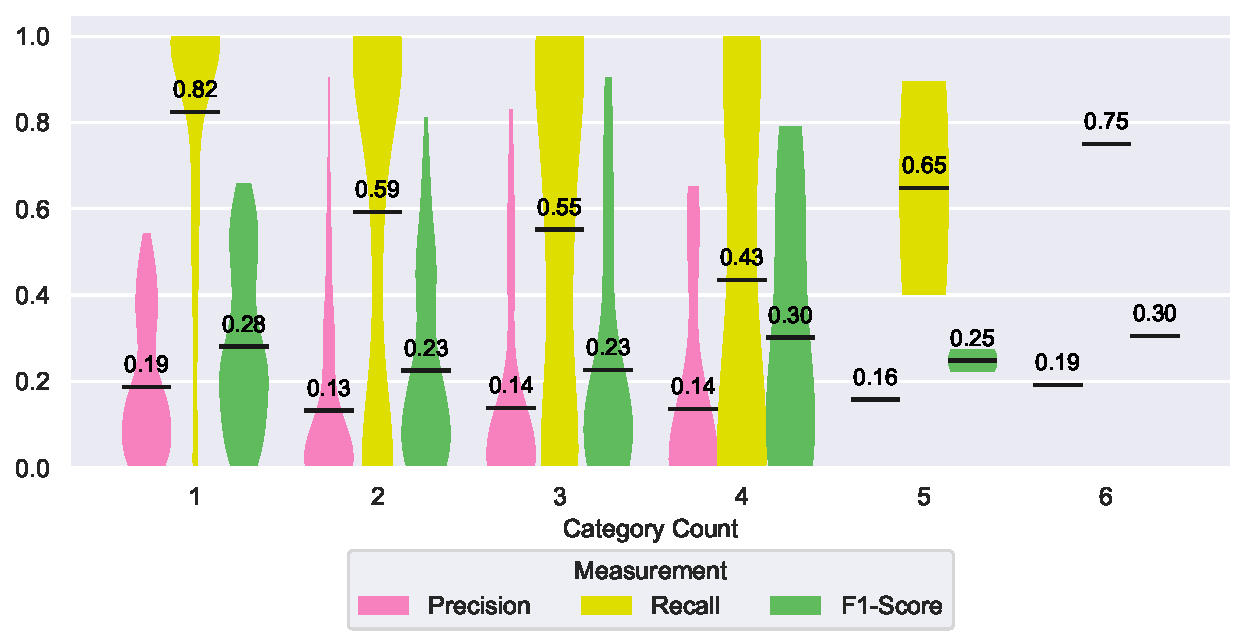
\includegraphics[width=\columnwidth,
		clip]{img/big-study/recall-precision-categorycount-KWS.pdf}
		\caption{structural category count
		in training and test sets.}
		\label{fig:recall-precision-categorycount-KWS}
\end{subfigure}
\caption{Precision, recall and F$_{1}$-score of chunk retrieval with
Keyword Search (KWS) compared by \ldots}
\end{figure*}


\Cref{fig:recall-precision-examplecount-KWS} presents precision,
recall and F$_{1}$-score of chunk retrieval using KWS for different
numbers of training examples.
The recall increases by about 12\% when
increasing the size of the training set to more than one example,
while the precision stays constant at around 16\%.
The F$_{1}$-score
stays around 26\%.

\Cref{fig:recall-precision-categorycount-KWS} shows the same
measurements for an increasing number of structural categories in the
training and test examples.
For more than one structural category in
the training and test examples the recall decreases by about 20\% and
the precision decreases about 6\%.
For more than two structural
categories no clear trend is visible in precision, recall or
F$_{1}$-score.

\subsection{Random Line Retrieval}
\label{sec:r:rlr}

In our evaluation, we compare against a baseline of randomly
picking lines from the build log.
Its results follow intuitive
expectations:
The precision ranges between 8\% and 5\%, the recall between 6\% and
8\%.
The size of the training set has no visible impact on either.
An larger number of structural categories within the training and
test sets decreased the precision of RLR from 7\% to 0\%, the recall
increases from 6\%, for one structural category present, to 11\%, for
three structural categories present and also drops to 0\% for more
structural categories.
Graphs of these results of the chunk retrieval with RLR
are included in our replication
package~\cite{brandt2020chunk-replication}.

\subsection{Comparison of All Techniques}
Next, we aggregate the results from
\Cref{sec:r:kws,sec:r:pbe,sec:r:cts,sec:r:rlr}.

\Cref{fig:success-partial-all} compares the success of chunk
retrievals differentiated by techniques in our study.
CTS and KWS
extract at least some of the desired lines in 79\% and 88.5\%
of the chunk retrieval runs.
With 38.25\%, KWS also has the highest proportion of fully
successful extractions, followed by PBE with 34.5\%.
PBE has the
lowest number of partial retrievals with only 18 out of 400 chunk
retrieval runs.

% % The averaged precision, recall and F$_{1}$-score f all techniques is
% % compared in Figure~\ref{fig:recall-precision-all}.
% The recall of PBE
% % has a high skew towards one and zero, meaning in most cases either
% % the retrieval is successful or no relevant lines are extracted at
% % all.
% PBE has the highest average precision with 95\%.
% Chunk
% % retrieval with CTS has the highest average F$_{1}$-score with 51\%
% % and the second highest recall with 46\%.
% KWS has the smallest
% % precision of the three chunk retrieval techniques.
% With 16\% it is
% % still higher than the precision of the RLR baseline with 7\%.
% KWS
% % has the highest recall of all techniques with 70\%.

\Cref{fig:recall-precision-singlecategory-all,fig:recall-precision-multicategory-all}
show the influence of a single structural category present in the
training examples compared to multiple categories present.
For more
than one category being present, the recall of PBE decreases greatly.
For CTS and KWS the values also decrease, while RLR is not affected by
the number of structural categories present.

\begin{figure}[!t]
		\centering
		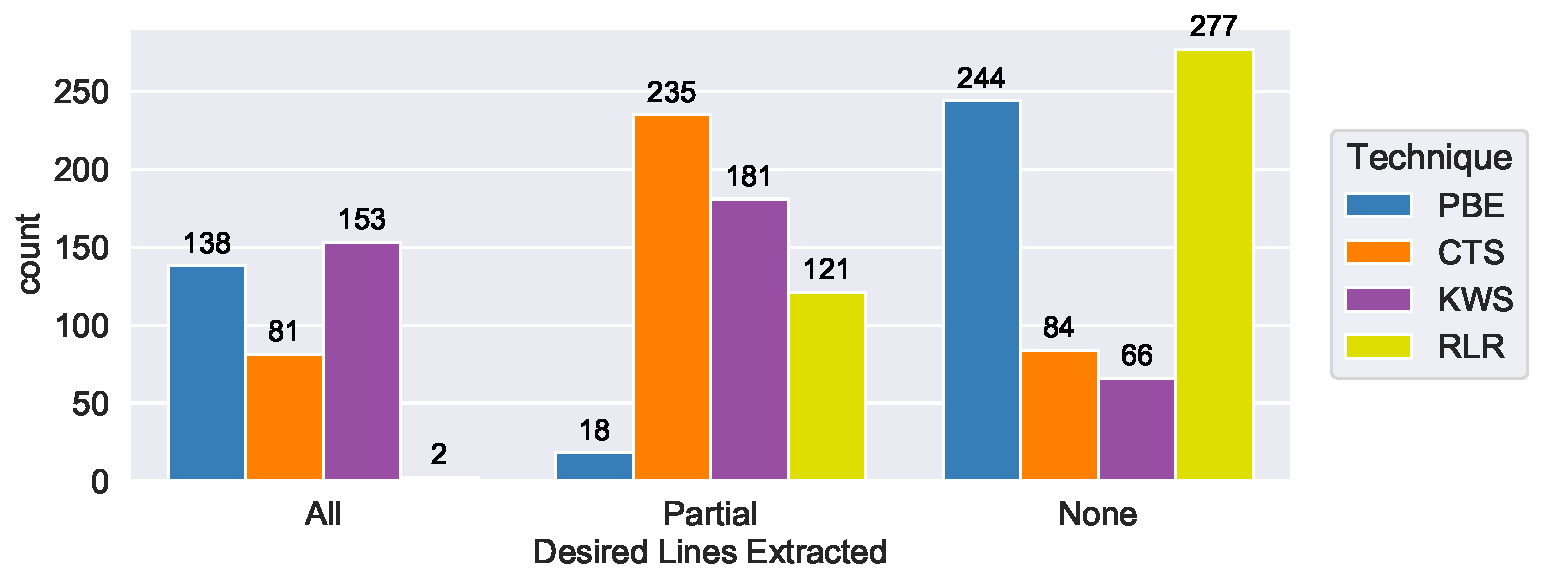
\includegraphics[width=\columnwidth,
		clip]{img/big-study/success-partial-all.pdf}
		\caption{Success of chunk retrievals for all techniques.}
		\label{fig:success-partial-all}
\end{figure}

\begin{figure*}
\centering
    \textbf{PBE, CTS, KWS, and RLR}\par\medskip
\begin{subfigure}[b]{\columnwidth}
		\centering
				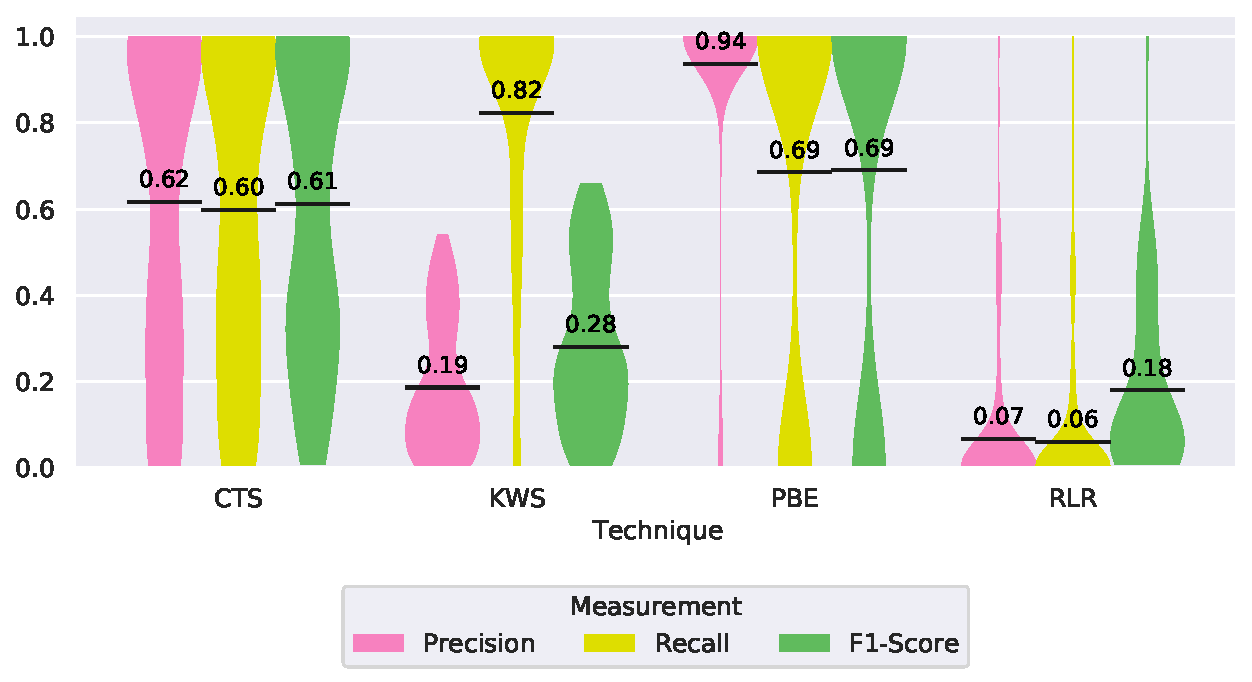
\includegraphics[width=\columnwidth,
				clip]{img/big-study/recall-precision-singlecategory-all.pdf}
		\caption{Training and test examples in 1
		structural category.}
		\label{fig:recall-precision-singlecategory-all}
\end{subfigure}\hspace{\fill}
\begin{subfigure}[b]{\columnwidth}
		\centering
				\centering
		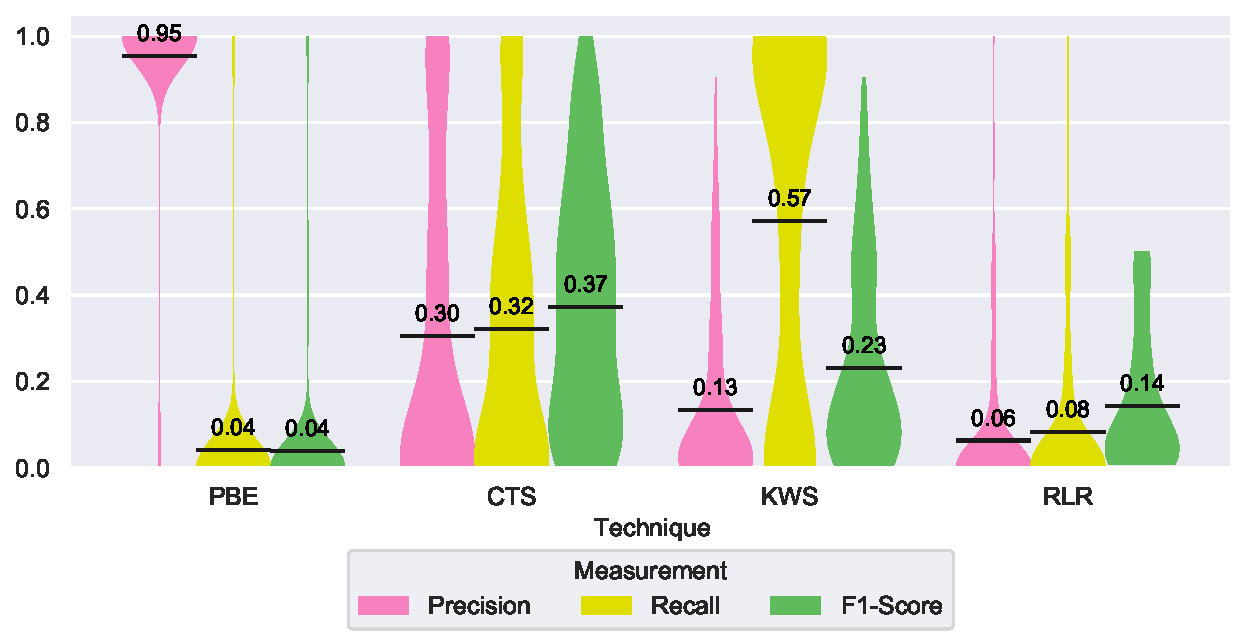
\includegraphics[width=\columnwidth,
		clip]{img/big-study/recall-precision-multicategory-all.pdf}
		\caption{Training and test examples in \textgreater
		1 structural
		category.}
		\label{fig:recall-precision-multicategory-all}
\end{subfigure}
\caption{Precision, recall and F$_{1}$-score of all
techniques compared, split by structural category count.}
\end{figure*}

\section{Discussion}
\label{sec:discussion}

For the interpretation of our study results we look at each chunk
retrieval technique separately and give recommendations for
which types of input build
logs, available training examples and consumption of the retrieved
output each technique is suited.
Following that, we discuss
which of these criteria should influence the decision to use a certain
chunk retrieval technique most.
Based on our empirical comparison, we present a
decision tree between the three techniques we investigated.

\subsection{Interpretation of Study Results}
\Cref{tab:single-technique-recommendations} summarizes the
recommendations which we discuss
in this section.

\begin{table}[tbp]
\resizebox{\columnwidth}{!}{%
\centering
\begin{tabular}{llll}
  \toprule
  & PBE & CTS & KWS \\
  \midrule
  Structural Categories & 1 & less is better & \makecell[l]{best 1 \\
  multiple okay} \\
  Training Set Size & 2 & no influence & 2 \\
  Precision & \makecell[l]{high \\ (if synthesis succeeds)} & medium &
  low \\
  Recall & \makecell[l]{high \\ (if synthesis succeeds)} & medium &
  high \\
  \makecell[l]{Confidence in \\ Output Correctness} & high & low &
  \makecell[l]{low (precision) \\ high (recall)} \\
  Output Consumption by & program & human & human \\
  \bottomrule
\end{tabular}%
}
\caption{Recommendations for each of the investigated chunk retrieval
techniques.}
\label{tab:single-technique-recommendations}
\end{table}

\subsubsection{Program Synthesis by Example (PBE)}

\noindent
\textbf{Configuration and Input}
Our study results show that chunk retrieval with PBE gives best
results when the training examples are structurally identical.
This is
because PROSE has difficulty synthesizing OR-based
programs~\cite{mayer2015user}.
PBE is thus suited to retrieve information
chunks that always have the same defining surrounding or internal
structure.
To extract for example the reason a build failed, the log
passage describing the failure would always have to be started and
ended the same way.

When the training examples are of the same structure, one or two
two examples are enough input for PROSE to synthesize a regular
expression program with good recall.
In our study, additional training
examples did not improve the chunk retrieval.
% In fact, unless they
% were in some sense redudant, adding training examples above that even
% hindered the applicability of PBE.

\noindent
\textbf{Retrieval Output Usage}
If the program synthesis succeeds and applying the regular expression
program yields an output, PBE has high precision and recall.
The tool
clearly identifies a failing synthesis or when the regular expression
finds no match on a build log.
Therefore, if PBE produces
an output, the user can have high confidence that it is the desired
output.
This preciseness makes output from PBE chunk retrieval
well-suited for machine consumption and therefore automatic on-ward
processing.

\subsubsection{Common Text Similarity (CTS)}
\noindent
\textbf{Configuration and Input}
Similar to PBE, chunk retrieval using CTS yields better results the
fewer structural categories are present in the training and test
examples.

The number of training examples had no noticeable influence on
precision or recall in our study.
Information retrieval techniques
like text similarity commonly learn on a higher number of examples
than used for our study.
Future work is needed to investigate how many
examples yield improvements in the chunk retrieval over a single
training example.

\noindent
\textbf{Retrieval Output Usage}
CTS has good precision and recall on average, though with a high
variation.
This means that the quality of an output by CTS is hard to
determine, which makes it unsuited for automatic  processing and requires
a human to further inspect and interpret the output.
This could include semi-automated procedures such as sending
developers an email with the extracted build failure reason.

\subsubsection{Keyword Search (KWS)}
\noindent
\textbf{Configuration and Input}
KWS has a higher recall than the two other techniques for multiple
structural categories present in the training and test examples.
This
makes KWS a good technique if there is little prior knowledge on how
the targeted log chunk is represented in the build log.
For the
example of extracting the reason the build failed, KWS is best suited
if a build can fail in various steps logged by different tools and no
pre-categorization of where the build failed is available.

Going from one to two training examples, KWS's recall improves
significantly.
However, further enlarging the training set
does not lead to further improvements.

\noindent
\textbf{Retrieval Output Usage}
While KWS has the highest recall of all three techniques, its
precision is the lowest.
The output of a chunk retrieval with KWS is
well-suited to be read by humans, but ill-suited for consumption by
automated tools.

\begin{figure}[tb]
		\centering
		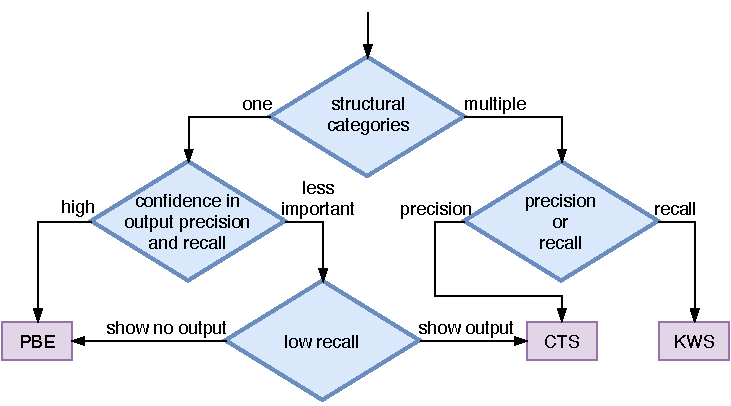
\includegraphics[width=\columnwidth,
		clip]{img/crt-recommendation.pdf}
		\caption{Our preliminary recommendation scheme for chunk
		retrieval techniques.}
		\label{fig:crt-recommendation}
\end{figure}

\subsection{Recommendation of Suitable Techniques}
After discussing the three chunk retrieval techniques separately we
now want to unify our results into one recommendation scheme.
Figure~\ref{fig:crt-recommendation} presents a decision tree
to answer our second research question;
If researchers or developers want to retrieve chunks from build logs,
they can follow the decision tree to identify the technique
suited best for their use case.
The decision tree is built up of questions
which either lead to more questions or to a leaf node containing a
recommended technique.

\begin{simplebox}[minipage boxed title*=-7cm]{Caveat!}
This is a preliminary hypothesis based on the results
from our comparison study.
The recommendations could therefore be
influenced by idiosyncrazies of our specific implementation of the
chunk retrieval techniques as well as the \emph{LogChunks}
data set.
\end{simplebox}

The first and most important aspect are the structural categories.
Are the targeted log chunks always presented in
the same structural way within the build logs? Then the information
chunks in all training examples and the analyzed build log are in the
same structural category.

If the information chunks are from multiple structural categories
and recall is more important than precision we recommend
to use KWS\@.
If precision is more important than recall to the user we
recommend CTS\@.
We also recommend CTS when the log chunks are
from one structural category, when the user does not require a high
confidence in the precision or recall of the outcome and when one
would rather have output with low recall instead of no output at all.
When the representations are from one structural category and the user
wishes a high confidence in the correctness of the output or prefers
no output over output with low recall, we recommend PBE\@.

As a final recommendation, one could create a ``super analyzer'' by
combining the different build log analysis techniques studied in this
paper.
Such a super analyzer would likely always first employ PBE
(because of its high accuracy), followed by a combination of CTS and
KWS\@.
Other than initial setup and training time, there should be no
downside to this approach if it is implemented in a transparent way to
the underlying technique: the output of the super analyzer could
include from which sub-tool it originated and thus facilitate
automatic on-ward processing or interpretation of the result.


\subsection{Examples of Using the Recommendation Scheme}
To illustrate how one would use our decision tree to find a suitable
chunk retrieval technique we describe two concrete examples: a software
team
wanting to monitor their build performance and a
researcher investigating why builds fail.

In our first example, a software development team wants to monitor
the performance of the phases within their CI build.
They are using
Travis CI, which measures the duration of build phases and documents
this within the build log.
As all log statements that report timing
measurements are formatted the same way, the targeted log chunks are
from one structural category.
Therefore the development team can use
PBE to retrieve the duration of a build phase.

In our second example, a researcher studies whether test failures
are caused by a small or by a large group of test cases.
They gather
CI build logs from various projects, which are their only available
data source.
The task of the researcher is to extract the names of the
failing test cases from each build log.
When they use our
recommendation scheme to select a chunk retrieval technique, they
first have to estimate how uniform the representation of the failing
test cases is in the investigated build logs.
As the researcher is
covering a wide range of test tools, the
log chunks they target are in various, non-predictable structural
representations.
The next question is whether they value precision
over recall.
As they have to manually inspect the results of both CTS
and KWS, they choose recall over precision to avoid having to inspect
the whole log in case the relevant information chunk was not
retrieved.
Therefore, our decision tree recommends to the researcher to use KWS\@.

In case the researcher wants to avoid manually inspecting the
retrieval results, they have to first separate the CI build logs
according to the test tool responsible for logging the test results.
Then the targeted log chunks are from one structural category and they
can use PBE, trained with examples from each test tool separately.

\section{Threats to Validity}
There are several threats to the validity of the conclusions of our
work.


\textbf{Implementation}
% TODO we need to say something about why we think that these
% limtiations do not actually harm our results
Our results depend on the implementation of the investigated chunk
retrieval techniques and the libraries we used.
Our implementation of
PBE is based on the program synthesis provided by PROSE\@.
The
idiosyncrazies of this framework influence our PBE results.
Other
frameworks similar to PROSE might have somewhat different strengths
and weaknesses.
For example, the need for examples from a single
structural category stems from the fact that PROSE cannot learn
regular expression programs with arbitrary boolean conjunctions and
disjunctions~\cite{mayer2015user}.
PROSE introduced this constraint to
keep the synthesis performance reasonable.
At the same time, this is
clearly a current theoretical challenge of all PBE implementations,
and we therefore attribute it to the technique itself, rather than the
specific implementation.

Our implementation of CTS is dependent on the library
{\tt text2vec}~\cite{text2vec2019webpage}
and the way it splits strings into word tokens.
On the other hand,
{\tt text2vec} is the de-facto standard library to do word embeddings
in R.
We intentionally chose a simple, minimally configured and tuned
approach to compare against.
Tuning the text similarity
meta-parameters more to the specific use case of chunk retrieval from
build logs would yield better chunk retrieval results.

\textbf{Data Set}
The outcomes of our comparison study are highly dependent on the build
logs from the \emph{LogChunks} data set.
It consists of build
logs from open source projects and therefore it is not clear whether
our results apply to industry projects that use build tools
not popular in open source development.
However, \emph{LogChunks} covers a wide array of build tools,
we believe that our findings can be generalized.
We collected build logs from Travis CI.
Yet, the format of the log chunk we chose
for our evaluation is not dependent on Travis CI\@.
This
is because the reason the build failed is described within the build
logs by the tools themselves and not the Travis CI environment.

\textbf{Training Set Size}
Especially the results for CTS might be influenced by the fact that we
only trained on one to five examples.
We chose this small training set
size as the training examples have to be provided per repository and
we expect a developer to not want to provide more examples than the
small numbers we evaluated on.
The fact that PBE and CTS performed best with already two training
examples shows that our training set size is large enough to
compare the three techniques we presented.

\textbf{Few Samples with Many Structural Categories}
Our comparison study shows fewer measurements with many structural
categories than with one structural category category
(50.25\% one, 33.75\% two, 13.75\% more than two).
This stems from the fact that we investigated the chunk retrieval
techniques on a real-world data set, where there were mostly few
structural categories within one project.
In addition, a third of the measurements were conducted with two
structural categories present and these already showed the negative
effect of the number of structural categories on the performance
of the chunk retrieval techniques.

\section{Future Work}

There are various future research opportunities based on our work:

\textbf{Systematic Survey of Industry Approaches for Build
Log Analysis}
Our survey is limited to academic work and articles.
However, handling build logs is a challenge for a wide range of
practitioners as well.
We propose to investigate the methods used in industry to analyze
build logs.
An example is the Jenkins \emph{build-failure-analyzer}
plugin~\cite{jenkins2020failure-analyzer} or automatically
inferred test results in Azure~\cite{azure2020inferred}.

\textbf{Further Analysis of \emph{LogChunks}}
We created the
\emph{LogChunks} data set \cite{brandt2020logchunks} specifically for
the comparative
study in this paper, though it can be the basis for various further
analyses of build log data.
The keywords, for example, can be
investigated to answer which keywords are used to search for the
reason the build failed within build logs.

\textbf{Cross-Repository Build Log Analysis}
We trained and
tested each chunk retrieval technique on examples from the same
repository.
We propose to analyze how techniques could be trained
across repositories, building the cornerstones for build
environment-agnostic analysis tools.

\textbf{Comparison with more Chunk Retrieval Techniques}
This
paper investigates the three chunk retrieval techniques PBE, CTS and
KWS\@.
Our study design can be reused to evaluate other build log
analysis techniques, such as the diff and information retrieval
approach by Amar et al.~\cite{amar2019mining}.

\textbf{Refinement of Retrieval Quality for each Technique} We
investigated basic configurations of existing techniques applied to
chunk retrieval from build logs.
In a next step, each of these
techniques could be refined to better approach the domain of build
logs.
The \emph{LogChunks} data set and our study results act as a
baseline to benchmark such technique improvements.
We propose the
following improvements:
\begin{itemize}
  \item \textbf{Custom Ranking and Tokens for PBE} The program
  synthesis through PROSE ranks possible programs according to
  what the user most likely intended.
  One could adapt the ranking
  rules provided by the FlashExtract DSL to fit common build log
  chunk retrieval tasks.
  FlashExtract includes special tokens when
  enumerating possible regular expressions.
  One could extend these
  with tokens found in build logs, such as ``-'',``='',``ERROR''
  or ``[OK''.
  \item \textbf{Meta-Parameter Optimization for CTS} Information
  retrieval techniques have various meta-parameters which can be
  optimized for the specific use
  case~\cite{panichella2016parameterizing}.
  We propose to further
  investigate improvements in preprocessing of the log text, in
  tokenization of the log lines into terms and in stop words
  lists.
\end{itemize}

\textbf{Usability Analysis of Chunk Retrieval Output}
Our
analysis of the output produced by the chunk retrieval focuses on
precision and recall.
The next step would be to investigate how useful these
outputs are to developers through controlled experiments.

\section{Conclusion}
\label{sec:conclusion-fw}
The goal of this paper was to support researchers and developers in
their decision on how to analyze build logs.
We conducted a systematic mapping study to uncover the
state-of-research on build log analysis.
We implemented	three promising chunk retrieval techniques and
compared them on our data set
\emph{LogChunks}, composed of 797 manually labeled build logs from a
broad range of 80 repositories.
Our results show that the structural
representation of the targeted information in the build logs is the
main factor to consider when choosing a suitable technique.
Secondary
factors are the desired confidence into recall and precision of the
produced output and whether precision or recall is more important for
the task at hand.

As a final recommendation, one could create a ``super analyzer'' by
combining the different build log analysis techniques studied in this
paper.
